\documentclass[]{beamer} 
\usetheme{Copenhagen}
\usecolortheme{default}

%\usepackage[ngerman]{babel}
\usepackage[latin1]{inputenc}
\usepackage{graphicx}
\usepackage{amsmath}
\usepackage{subfigure}
\usepackage{hyperref}

%Einige n�tzliche LaTeX-Makros
%(c) 2005/2006 by Jan W. Krieger
%  jan@jkrieger.de --- http://www.jkrieger.de/
%FREEWARE - you are free to use this software or any 
%           portion of it in any way you want to. 
%           Although I would be lucky to receive a message 
%           if you changed something or found this software 
%           useful...

\usepackage{ifthen}

%ge�ndertes Label-Makro, damit man auch mit hyperref auf Labels verweisen kann!
\newcommand{\jlabel}[1]{\hypertarget{#1}{}\label{#1}}


% Farb-Definitionen f�r meinen pers�nlichen Dokument-Stil
\ifthenelse{\isundefined{\hyperpage}}{}{\newcommand{\glossaryentry}[2]{\item #1 \hyperpage{#2}}}


% Befehle f�r Index-Erstellung
\newcommand{\itindex}[1]{{{\index{#1}}#1}} % Index-Eintrag im Flie�text. Es wird der Eintrag selbe auch ausgegeben.
\newcommand{\itindexbf}[1]{{\textbf{{\index{#1}}#1}}}
\newcommand{\itindexit}[1]{{\textit{{\index{#1}}#1}}}


%zur Fehlerbehebung bei Verwendung mit TeXnicCenter 4 beta
\newcommand{\p}{\\[3mm]}
\newcommand{\script}{\scriptsize}


% Vektoren
\newcommand{\twovector}[2]{\begin{pmatrix} #1 \\ #2 \end{pmatrix}} % Vektor mit zwei zwei Eintr�gen
\newcommand{\smalltwovector}[2]{\left(\begin{smallmatrix} #1 \\ #2 \end{smallmatrix}\right)} 
\newcommand{\jvector}[3]{\begin{array}{c} #1 \\ #2 \\ #3 \end{array}} % Vektor mit drei Eintr�gen
\newcommand{\threevector}[3]{\begin{pmatrix} #1 \\ #2 \\ #3 \end{pmatrix}} % Vektor mit drei Eintr�gen
\newcommand{\smallthreevector}[3]{\left(\begin{smallmatrix} #1 \\ #2 \\ #3 \end{smallmatrix}\right)} % kleiner Vektor mit drei Eintr�gen
\newcommand{\fourvector}[4]{\begin{pmatrix} #1 \\ #2 \\ #3 \\ #4 \end{pmatrix}} % Vektor mit vier Eintr�gen
\newcommand{\smallfourvector}[4]{\left(\begin{smallmatrix} #1 \\ #2 \\ #3 \\ #4\end{smallmatrix}\right)}% kleiner Vektor mit vier Eintr�gen
 \newcommand{\vecn}[2]{\begin{pmatrix} #1 \\\vdots\\ #2 \end{pmatrix}} % Vektor der Form (x_1 ... x_n)
\newcommand{\vecxnsmall}{\left(\begin{smallmatrix} x_1 \\ \vdots \\ x_n \end{smallmatrix}\right)}
\newcommand{\vecynsmall}{\left(\begin{smallmatrix} y_1 \\ \vdots \\ y_n \end{smallmatrix}\right)}
\newcommand{\vecxntsmall}{\left(x_1,\ldots,x_n\right)}
\newcommand{\vecyntsmall}{\left(y_1,\ldots,y_n\right)}

% Matritzen
\newcommand{\fourmatrix}[4]{\begin{pmatrix} #1 & #2 \\ #3 & #4 \end{pmatrix}} % 2x2-Matrix

% spezielle Matritzen
\newcommand{\matAmnsmall}{\left(\begin{smallmatrix} a_{11} & \ldots & a_{1n}\\ \vdots & \ddots & \vdots \\	a_{n1} & \ldots & a_{nn}\end{smallmatrix}\right)} % kleine nxn-Matrix mit Eintr�gen a_ij
\newcommand{\matBmnsmall}{\left(\begin{smallmatrix} b_{11} & \ldots & b_{1n}\\ \vdots & \ddots & \vdots \\	b_{n1} & \ldots & b_{nn}\end{smallmatrix}\right)} % kleine nxn-Matrix mit Eintr�gen b_ij
\newcommand{\matCmnsmall}{\left(\begin{smallmatrix} c_{11} & \ldots & c_{1n}\\ \vdots & \ddots & \vdots \\	c_{n1} & \ldots & c_{nn}\end{smallmatrix}\right)}% kleine nxn-Matrix mit Eintr�gen c_ij
\newcommand{\matTmnsmall}{\left(\begin{smallmatrix} t_{11} & \ldots & t_{1n}\\ \vdots & \ddots & \vdots \\	t_{n1} & \ldots & t_{nn}\end{smallmatrix}\right)}% kleine nxn-Matrix mit Eintr�gen t_ij
\newcommand{\matAmn}{\left(\begin{array}{cccc}a_{11} & a_{12} & \ldots & a_{1n}\\a_{21} & a_{22} & \ldots & a_{2n}\\\vdots &\vdots &\ddots & \vdots\\a_{m1} & a_{m2} & \ldots & a_{mn}\\\end{array}\right)} % mxn-Matrix mit Eintr�gen a_ij
\newcommand{\matAnn}{\left(\begin{array}{cccc}a_{11} & a_{12} & \ldots & a_{1n}\\a_{21} & a_{22} & \ldots & a_{2n}\\\vdots & & & \vdots\\a_{n1} & a_{n2} & \ldots & a_{nn}\\\end{array}\right)} % nxn-Matrix mit Eintr�gen a_ij
\newcommand{\matEnBig}{\left(\begin{array}{cccc}1 & 0 & \ldots & 0\\0 & 1 & \ddots & \vdots\\\vdots & \ddots & \ddots& 0\\0 & \ldots & 0 & 1\\\end{array}\right)} % gro�e nxn-Einheitsmatrix
\newcommand{\matEn}{\left(\begin{array}{cc}1 & \mathbf{0} \\ \mathbf{0} & 1\end{array}\right)} % Einheitsmatrix
\newcommand{\matDiag}[2]{\begin{pmatrix}#1 &  & \mathbf{0}\\  & \ddots & \\ \mathbf{0} &  & #2\end{pmatrix}} % Diagonalmatrix mit Eintr�gen x_1..x_2 auf der Diagonalen
\newcommand{\matThreeDiag}[3]{\begin{pmatrix}#1 & 0 & 0\\ 0 & #2 & 0\\ 0 & 0 & #3\end{pmatrix}} % 3x3-Diagonalmatrix
\newcommand{\matTriangle}[2]{\begin{pmatrix}#1 & \cdots & \\  & \ddots & \vdots\\ \mathbf{0}&  & #2\end{pmatrix}} % rechte obere Dreiecksamtrix

%Determinanten
\newcommand{\fourdet}[4]{\begin{vmatrix} #1 & #2 \\ #3 & #4 \end{vmatrix}}

% Real- und Imagin�rteil-Operatoren
\renewcommand{\Re}{\mathrm{Re}\;}
\renewcommand{\Im}{\mathrm{Im}\;}


% Darstellung von Einheiten
\newcommand{\unit}[1]{\:\mathrm{#1}}
\newcommand{\unitf}[2]{\:\mathrm{\frac{#1}{#2}}}


\newcommand{\const}{{\text{const}}}


% Differentialbr�che
\newcommand{\pfrac}[2]{\frac{\partial #1}{\partial #2}}  % partielles Differential
\newcommand{\fracpd}[2]{\frac{\partial #1}{\partial #2}} % partielles Differential
\newcommand{\fracppd}[2]{\frac{\partial^2 #1}{\partial #2^2}}  % zweite partielle 
\newcommand{\fracd}[2]{\frac{\mathrm{d} #1}{\mathrm{d} #2}} % partielles Differential
\newcommand{\fracdd}[2]{\frac{\mathrm{d}^2 #1}{\mathrm{d} #2^2}}  % zweite partielle 


\newcommand{\dd}{\mathrm{d}}  
\newcommand{\ii}{\mathrm{i}}  

% Blackboard-Font: Bezeichnungen f�r Mengen
\newcommand{\bbone}{\mathds{1}}  % mathds ben�tigt das Package "dsfont"
\newcommand{\C}{\mathbb{C}}
\newcommand{\K}{\mathbb{K}}
\newcommand{\N}{\mathbb{N}}
\newcommand{\bP}{\mathbb{P}}
\newcommand{\Q}{\mathbb{Q}}
\newcommand{\R}{\mathbb{R}}
\newcommand{\Z}{\mathbb{Z}}
\newcommand{\bbA}{\mathbb{A}}
\newcommand{\bbB}{\mathbb{B}}
\newcommand{\bbC}{\mathbb{C}}
\newcommand{\bbD}{\mathbb{D}}
\newcommand{\bbE}{\mathbb{E}}
\newcommand{\bbF}{\mathbb{F}}
\newcommand{\bbG}{\mathbb{G}}
\newcommand{\bbH}{\mathbb{H}}
\newcommand{\bbI}{\mathbb{I}}
\newcommand{\bbJ}{\mathbb{J}}
\newcommand{\bbK}{\mathbb{K}}
\newcommand{\bbL}{\mathbb{L}}
\newcommand{\bbM}{\mathbb{M}}
\newcommand{\bbN}{\mathbb{N}}
\newcommand{\bbO}{\mathbb{O}}
\newcommand{\bbP}{\mathbb{P}}
\newcommand{\bbQ}{\mathbb{Q}}
\newcommand{\bbR}{\mathbb{R}}
\newcommand{\bbS}{\mathbb{S}}
\newcommand{\bbT}{\mathbb{T}}
\newcommand{\bbU}{\mathbb{U}}
\newcommand{\bbV}{\mathbb{V}}
\newcommand{\bbW}{\mathbb{W}}
\newcommand{\bbX}{\mathbb{X}}
\newcommand{\bbY}{\mathbb{Y}}
\newcommand{\bbZ}{\mathbb{Z}}


% spezielle Mengen R^n etc.
\newcommand{\Knn}{\mathbb{K}^{n\times n}}
\newcommand{\Kmn}{\mathbb{K}^{m\times n}}
\newcommand{\Rnn}{\mathbb{R}^{n\times n}}
\newcommand{\Rmn}{\mathbb{R}^{m\times n}}
\newcommand{\Rmm}{\mathbb{R}^{m\times m}}
\newcommand{\Kn}{\mathbb{K}^n}
\newcommand{\Rn}{\mathbb{R}^n}
\newcommand{\Rthree}{\mathbb{R}^3}
\newcommand{\Km}{\mathbb{K}^m}
\newcommand{\Rm}{\mathbb{R}^m}
\newcommand{\HM}{\mathcal{H}(M)}
\newcommand{\KX}{K\left[X\right]} %Menge der Polynome �ber X (???)
\newcommand{\jset}[2]{\bigl\{ #1 \bigl| #2 \bigr.\bigr\}} % Menge aller Elemente #1 mit Eigenschaft #2
\newcommand{\mCab}{{\cC}\left[a,b\right]} % C[a,b]
\newcommand{\Cab}{{$\mCab$}} % Cab au�erhalb Mathe-Modus


% Gro�-Buchstaben im mathcal-Font
\newcommand{\cA}{\mathcal{A}}
\newcommand{\cB}{\mathcal{B}}
\newcommand{\cC}{\mathcal{C}}
\newcommand{\cD}{\mathcal{D}}
\newcommand{\cE}{\mathcal{E}}
\newcommand{\cF}{\mathcal{F}}
\newcommand{\cG}{\mathcal{G}}
\newcommand{\cH}{\mathcal{H}}
\newcommand{\cI}{\mathcal{I}}
\newcommand{\cJ}{\mathcal{J}}
\newcommand{\cK}{\mathcal{K}}
\newcommand{\calL}{\mathcal{L}}
\newcommand{\cL}{\mathcal{L}}
\newcommand{\cM}{\mathcal{M}}
\newcommand{\cN}{\mathcal{N}}
\newcommand{\cO}{\mathcal{O}}
\newcommand{\cP}{\mathcal{P}}
\newcommand{\cQ}{\mathcal{Q}}
\newcommand{\cR}{\mathcal{R}}
\newcommand{\cS}{\mathcal{S}}
\newcommand{\cT}{\mathcal{T}}
\newcommand{\cU}{\mathcal{U}}
\newcommand{\cV}{\mathcal{V}}
\newcommand{\cW}{\mathcal{W}}
\newcommand{\bX}{\mathbf{X}}
\newcommand{\bY}{\mathbf{Y}}
\newcommand{\cZ}{\mathcal{Z}}

% Operatoren als Vektoren (Nabla ...)
\newcommand{\vnabla}{\vec{\nabla}}

% ausgew�hlte griechische Buchstaben als Vektoren
\newcommand{\valpha}{\vec{\alpha}}
\newcommand{\vbeta}{\vec{\beta}}
\newcommand{\vgamma}{\vec{\gamma}}
\newcommand{\vdelta}{\vec{\delta}}
\newcommand{\vepsilon}{\vec{\epsilon}}
\newcommand{\vtau}{\vec{\tau}}
\newcommand{\vmu}{\vec{\mu}}
\newcommand{\vphi}{\vec{\phi}}
\newcommand{\vpi}{\vec{\pi}}
\newcommand{\vPsi}{\vec{\Psi}}
\newcommand{\vchi}{\vec{\chi}}
\newcommand{\vvarphi}{\vec{\varphi}}
\newcommand{\veta}{\vec{\eta}}
\newcommand{\viota}{\vec{\iota}}
\newcommand{\vkappa}{\vec{\kappa}}
\newcommand{\vlambda}{\vec{\lambda}}
\newcommand{\vnu}{\vec{\nu}}
\newcommand{\vgo}{\vec{\o}}
\newcommand{\vvarpi}{\vec{\varpi}}
\newcommand{\vtheta}{\vec{\theta}}
\newcommand{\vvartheta}{\vec{\vartheta}}
\newcommand{\vrho}{\vec{\rho}}
\newcommand{\vsigma}{\vec{\sigma}}
\newcommand{\vvarsigma}{\vec{\varsigma}}
\newcommand{\vupsilon}{\vec{\upsilon}}
\newcommand{\vomega}{\vec{\omega}}
\newcommand{\vxi}{\vec{\xi}}
\newcommand{\vpsi}{\vec{\psi}}
\newcommand{\vzeta}{\vec{\zeta}}



% Gro�buchstaben als Vektoren
\newcommand{\vA}{\vec{A}}
\newcommand{\vB}{\vec{B}}
\newcommand{\vC}{\vec{C}}
\newcommand{\vD}{\vec{D}}
\newcommand{\vE}{\vec{E}}
\newcommand{\vF}{\vec{F}}
\newcommand{\vG}{\vec{G}}
\newcommand{\vH}{\vec{H}}
\newcommand{\vI}{\vec{I}}
\newcommand{\vJ}{\vec{J}}
\newcommand{\vK}{\vec{K}}
\newcommand{\vL}{\vec{L}}
\newcommand{\vM}{\vec{M}}
\newcommand{\vN}{\vec{N}}
\newcommand{\vO}{\vec{O}}
\newcommand{\vP}{\vec{P}}
\newcommand{\vQ}{\vec{Q}}
\newcommand{\vR}{\vec{R}}
\newcommand{\vS}{\vec{S}}
\newcommand{\vT}{\vec{T}}
\newcommand{\vU}{\vec{U}}
\newcommand{\vV}{\vec{V}}
\newcommand{\vW}{\vec{W}}
\newcommand{\vX}{\vec{X}}
\newcommand{\vY}{\vec{Y}}
\newcommand{\vZ}{\vec{Z}}


% Kleinbuchstaben als Vektoren
\newcommand{\va}{\vec{a}}
\newcommand{\vb}{\vec{b}}
\newcommand{\vc}{\vec{c}}
\newcommand{\vd}{\vec{d}}
\newcommand{\ve}{\vec{e}}
\newcommand{\vf}{\vec{f}}
\newcommand{\vg}{\vec{g}}
\newcommand{\vh}{\vec{h}}
\newcommand{\vi}{\vec{i}}
\newcommand{\vj}{\vec{j}}
\newcommand{\vk}{\vec{k}}
\newcommand{\vl}{\vec{l}}
\newcommand{\vm}{\vec{m}}
\newcommand{\vn}{\vec{n}}
\newcommand{\vo}{\vec{o}}
\newcommand{\vp}{\vec{p}}
\newcommand{\vq}{\vec{q}}
\newcommand{\vr}{\vec{r}}
\newcommand{\vs}{\vec{s}}
\newcommand{\vt}{\vec{t}}
\newcommand{\vu}{\vec{u}}
\newcommand{\vv}{\vec{v}}
\newcommand{\vw}{\vec{w}}
\newcommand{\vx}{\vec{x}}
\newcommand{\vy}{\vec{y}}
\newcommand{\vz}{\vec{z}}


%Formatierung von Matritzen
\newcommand{\mat}[1]{\mathrm{\mathbf{#1}}}


% Gro�buchstaben als Matritzen
\newcommand{\mOne}{\mat{\mathds{1}}} % ben�tigt mathds-Package
\newcommand{\mA}{\mat{A}}
\newcommand{\mB}{\mat{B}}
\newcommand{\mC}{\mat{C}}
\newcommand{\mD}{\mat{D}}
\newcommand{\mE}{\mat{E}}
\newcommand{\mF}{\mat{F}}
\newcommand{\mG}{\mat{G}}
\newcommand{\mH}{\mat{H}}
\newcommand{\mI}{\mat{I}}
\newcommand{\mJ}{\mat{J}}
\newcommand{\mK}{\mat{K}}
\newcommand{\mL}{\mat{L}}
\newcommand{\mM}{\mat{M}}
\newcommand{\mN}{\mat{N}}
\newcommand{\mO}{\mat{O}}
\newcommand{\mP}{\mat{P}}
\newcommand{\mQ}{\mat{Q}}
\newcommand{\mR}{\mat{R}}
\newcommand{\mS}{\mat{S}}
\newcommand{\mT}{\mat{T}}
\newcommand{\mU}{\mat{U}}
\newcommand{\mV}{\mat{V}}
\newcommand{\mW}{\mat{W}}
\newcommand{\mX}{\mat{X}}
\newcommand{\mY}{\mat{Y}}
\newcommand{\mZ}{\mat{Z}}

\newcommand{\msigma}{\mat{\sigma}}



% Gr��en mit Hut
\newcommand{\hx}{\hat{x}}
\newcommand{\hlambda}{\hat{\lambda}}
\newcommand{\hy}{\hat{y}}

% h�ufige Grenz�berg�nge
\newcommand{\limninfty}{\lim\limits_{n\rightarrow\infty}} % lim n -> infty
\newcommand{\limkinfty}{\lim\limits_{k\rightarrow\infty}} % lim k -> infty
\newcommand{\liminfninfty}{\liminf\limits_{n\rightarrow\infty}} % liminf n-> infty
\newcommand{\liminfkinfty}{\liminf\limits_{k\rightarrow\infty}} % liminf k-> infty
\newcommand{\limsupninfty}{\limsup\limits_{n\rightarrow\infty}} % limsup n-> infty
\newcommand{\limsupkinfty}{\limsup\limits_{k\rightarrow\infty}} % limsup k-> infty
\newcommand{\supnN}{\sup\limits_{n\in\N}} % sup n in N
\newcommand{\infnN}{\sup\limits_{n\in\N}} % inf n in N
\newcommand{\ninfty}{n\rightarrow\infty} % n -> infty
\newcommand{\kinfty}{k\rightarrow\infty} % k -> infty
\newcommand{\epsilonzero}{\epsilon\rightarrow0} % epsilon -> 0
\newcommand{\epsilonnull}{\epsilon\rightarrow0} % epsilon -> 0
\newcommand{\hzero}{h\rightarrow0} % h -> 0
\newcommand{\hnull}{h\rightarrow0} % h -> 0

% h�ufige Summationen
\newcommand{\sumknullinfty}{\sum\limits_{k=0}^\infty}
\newcommand{\sumnnullinfty}{\sum\limits_{n=0}^\infty}
\newcommand{\sumkzeroinfty}{\sum\limits_{k=0}^\infty}
\newcommand{\sumnzeroinfty}{\sum\limits_{n=0}^\infty}
\newcommand{\sumkoneinfty}{\sum\limits_{k=1}^\infty}
\newcommand{\sumkonen}{\sum\limits_{k=1}^n}
\newcommand{\sumkonem}{\sum\limits_{k=1}^m}
\newcommand{\sumionen}{\sum\limits_{i=1}^n}
\newcommand{\sumjonen}{\sum\limits_{j=1}^n}
\newcommand{\sumionem}{\sum\limits_{i=1}^m}
\newcommand{\sumnoneinfty}{\sum\limits_{n=1}^\infty}

% diverse Operatoren/Funktionen etc.

% lineare Algebra (Normen etc.)
\newcommand{\sabs}[1]{{|#1|}} % Absolut-Betrag
\newcommand{\abs}[1]{\left|#1\right|} % Absolut-Betrag
\newcommand{\bigabs}[1]{\bigl|#1\bigr|} % Absolut-Betrag, gro�
\newcommand{\absa}[1]{\left|#1\right|_a}
\newcommand{\absi}[1]{\left|#1\right|_i}
\newcommand{\norm}[2][]{\left\|#2\right\|_{#1}} % Norm
\newcommand{\normmax}[1]{\left\|#1\right\|_{\infty}} % infty-Norm
\newcommand{\normltwo}[1]{\left\|#1\right\|_{2}} % L2-Norm
\newcommand{\transp}[1]{{#1}^t} % Transposition
\newcommand{\skalarp}[2]{\langle #1, #2 \rangle}

% spezielle Befehle: Physik
\newcommand{\lorentz}{\textsc{Lorentz}}
\newcommand{\einstein}{\textsc{Einstein}}
\newcommand{\smallmetric}{\left(\begin{smallmatrix}1 & & &\mathbf{0}\\ & -1 & &\\ & & -1 &\\\mathbf{0} & & &-1\\\end{smallmatrix}\right)} % Metrik der spec. Rel.
\newcommand{\poisson}[2]{\left\{{#1},{#2}\right\}}

%Quantenmechanische Bra-Ket-Notation
\newcommand{\bra}[1]{\langle{#1}|}
\newcommand{\ket}[1]{|{#1}\rangle}
\newcommand{\braOPket}[3]{\langle #1|\hat{#2}| #3\rangle}
\newcommand{\braOPvket}[3]{\langle #1|\hat{\vec{#2}}| #3\rangle}
\newcommand{\braopket}[3]{\langle #1| #2 | #3\rangle}
\newcommand{\braket}[2]{\langle #1 | #2 \rangle}
\newcommand{\ketbra}[2]{\ket{#1}\bra{#2}}
\newcommand{\qmskalar}[2]{\langle #1, #2 \rangle}
\newcommand{\OP}[1]{\hat{\mathrm{#1}}}
\newcommand{\OPv}[1]{\hat{\vec{\mathrm{#1}}}}
\newcommand{\obs}[1]{\mathcal{#1}}
\newcommand{\obsv}[1]{\vec{\mathcal{#1}}}
\newcommand{\commutator}[2]{[#1, #2]}
\newcommand{\commutatorOP}[2]{[\hat{#1}, \hat{#2}]}
\newcommand{\commutatorOPv}[2]{[\hat{\vec{#1}}, \hat{#2}]}
\newcommand{\acommutator}[2]{\{#1, #2\}}
\newcommand{\acommutatorOP}[2]{\{\hat{#1}, \hat{#2}\}}
\newcommand{\acommutatorOPv}[2]{\{\hat{\vec{#1}}, \hat{#2}\}}
\newcommand{\smean}[1]{\bigl\langle #1\bigr\rangle}
\newcommand{\mean}[1]{\left\langle #1\right\rangle}
\newcommand{\meanOP}[1]{\langle\hat{#1}\rangle}
\newcommand{\meanOPv}[1]{\langle\hat{\vec{#1}}\rangle}
\newcommand{\prob}[1]{\bP\left({#1}\right)}
\newcommand{\tp}{\otimes}

\newcommand{\ketupsdown}{\ket{\uparrow/\downarrow}}
\newcommand{\braupsdown}{\bra{\uparrow/\downarrow}}

\newcommand{\ketupup}{\ket{\uparrow\uparrow}}
\newcommand{\braupup}{\bra{\uparrow\uparrow}}
\newcommand{\ketupdown}{\ket{\uparrow\downarrow}}
\newcommand{\braupdown}{\bra{\uparrow\downarrow}}
\newcommand{\ketdownup}{\ket{\downarrow\uparrow}}
\newcommand{\bradownup}{\bra{\downarrow\uparrow}}
\newcommand{\ketdowndown}{\ket{\downarrow\downarrow}}
\newcommand{\bradowndown}{\bra{\downarrow\downarrow}}
\newcommand{\ketup}{\ket{\uparrow}}
\newcommand{\braup}{\bra{\uparrow}}
\newcommand{\ketdown}{\ket{\downarrow}}
\newcommand{\bradown}{\bra{\downarrow}}
\newcommand{\ketnlm}{\ket{nlm}}
\newcommand{\branlm}{\bra{nlm}}
\newcommand{\ketp}{\ket{p}}
\newcommand{\ketq}{\ket{q}}
\newcommand{\ketn}{\ket{n}}
\newcommand{\keta}{\ket{a}}
\newcommand{\braa}{\bra{a}}
\newcommand{\ketb}{\ket{b}}
\newcommand{\brab}{\bra{b}}
\newcommand{\ketr}{\ket{r}}
\newcommand{\brar}{\bra{r}}
\newcommand{\ketpsi}{\ket{\psi}}
\newcommand{\ketphi}{\ket{\phi}}
\newcommand{\brap}{\bra{p}}
\newcommand{\braq}{\bra{q}}
\newcommand{\bran}{\bra{n}}
\newcommand{\brapsi}{\bra{\psi}}
\newcommand{\braphi}{\bra{\phi}}
\newcommand{\OPA}{\OP{A}}
\newcommand{\OPvA}{\OPv{A}}
\newcommand{\OPa}{\OP{a}}
\newcommand{\OPadagger}{{\OP{a}^\dagger}}
\newcommand{\OPad}{\OPadagger}
\newcommand{\OPB}{\OP{B}}
\newcommand{\OPC}{\OP{C}}
\newcommand{\OPD}{\OP{D}}
\newcommand{\OPE}{\OP{E}}
\newcommand{\OPF}{\OP{F}}
\newcommand{\OPG}{\OP{G}}
\newcommand{\OPH}{\OP{H}}
\newcommand{\OPI}{\OP{I}}
\newcommand{\OPJ}{\OP{J}}
\newcommand{\OPJs}{\OP{J}^2}
\newcommand{\OPJx}{\OP{J}_x}
\newcommand{\OPJpm}{\OP{J}_{\pm}}
\newcommand{\OPJmp}{\OP{J}_{\mp}}
\newcommand{\OPJp}{\OP{J}_{+}}
\newcommand{\OPJm}{\OP{J}_{-}}
\newcommand{\OPJy}{\OP{J}_y}
\newcommand{\OPJz}{\OP{J}_z}
\newcommand{\OPJv}{\OPv{J}}
\newcommand{\OPJvs}{\OPv{J}^2}
\newcommand{\OPvJ}{\OPJv}
\newcommand{\OPK}{\OP{K}}
\newcommand{\OPk}{\OP{k}}
\newcommand{\OPL}{\OP{L}}
\newcommand{\OPLs}{\OP{L}^2}
\newcommand{\OPLp}{\OP{L}_{+}}
\newcommand{\OPLpm}{\OP{L}_{\pm}}
\newcommand{\OPLmp}{\OP{L}_{\mp}}
\newcommand{\OPLm}{\OP{L}_{-}}
\newcommand{\OPLx}{\OP{L}_x}
\newcommand{\OPLy}{\OP{L}_y}
\newcommand{\OPLz}{\OP{L}_z}
\newcommand{\OPLv}{\OPv{L}}
\newcommand{\OPvL}{\OPLv}
\newcommand{\OPLvs}{\OPv{L}^2}
\newcommand{\OPM}{\OP{M}}
\newcommand{\OPN}{\OP{N}}
\newcommand{\OPn}{\OP{n}}
\newcommand{\OPO}{\OP{O}}
\newcommand{\OPP}{\OP{P}}
\newcommand{\OPvP}{\OPv{P}}
\newcommand{\OPQ}{\OP{Q}}
\newcommand{\OPvQ}{\OPv{Q}}
\newcommand{\OPp}{\OP{p}}
\newcommand{\OPq}{\OP{q}}
\newcommand{\OPR}{\OP{R}}
\newcommand{\OPr}{\OP{r}}
\newcommand{\OPvR}{\OPv{R}}
\newcommand{\OPS}{\OP{S}}
\newcommand{\OPSs}{\OP{S}^2}
\newcommand{\OPSp}{\OP{S}_{+}}
\newcommand{\OPSpm}{\OP{S}_{\pm}}
\newcommand{\OPSmp}{\OP{S}_{\mp}}
\newcommand{\OPSm}{\OP{S}_{-}}
\newcommand{\OPSx}{\OP{S}_x}
\newcommand{\OPSy}{\OP{S}_y}
\newcommand{\OPSz}{\OP{S}_z}
\newcommand{\OPSv}{\OPv{S}}
\newcommand{\OPvS}{\OPSv}
\newcommand{\OPSvs}{\OPv{S}^2}

\newcommand{\OPT}{\OP{T}}
\newcommand{\OPU}{\OP{U}}
\newcommand{\OPV}{\OP{V}}
\newcommand{\OPW}{\OP{W}}
\newcommand{\OPX}{\OP{X}}
\newcommand{\OPvX}{\OPv{X}}
\newcommand{\OPY}{\OP{Y}}
\newcommand{\OPZ}{\OP{Z}}
\newcommand{\OPx}{\OP{x}}
\newcommand{\OPy}{\OP{y}}
\newcommand{\OPz}{\OP{z}}
\newcommand{\OPPi}{\OP{\Pi}}



\newcommand{\rhoMK}{{\rho_{\txt{MK}}}}
\newcommand{\rhoK}{{\rho_{\txt{K}}}}
\newcommand{\rhoGK}{{\rho_{\txt{GK}}}}
\newcommand{\OPrhoMK}{{\OP{\rho}_{\txt{MK}}}}
\newcommand{\OPrhoK}{{\OP{\rho}_{\txt{K}}}}
\newcommand{\OPrhoGK}{{\OP{\rho}_{\txt{GK}}}}
\newcommand{\OPrho}{{\OP{\rho}}}

% spezielle Befehle: theoretische Informatik: Operatoren etc.
\newcommand{\defined}{\!\!\downarrow} % gr��e ist definiert (Pfeil nach unten)
\newcommand{\mundefined}{\!\!\uparrow} % gr��e ist nicht definiert (Pfeil nach oben)
\newcommand{\FPRIM}{F(\text{PRIM})} % Klasse der primitiv rekursiven Funktioenn
\newcommand{\FREK}{F(\text{REK})} % Klasse der rekursiven Funktionen
\newcommand{\RETURN}{\textbf{return}\ }
\newcommand{\xk}{x^{(k)}}
\newcommand{\xkpone}{x^{(k+1)}}
\newcommand{\xkmone}{x^{(k-1)}}
\newcommand{\xn}{x^{(n)}}
%\newcommand{\xl}{x^{(l)}}
\newcommand{\xj}{x^{(j)}}
\newcommand{\ei}{e^{(i)}}
\newcommand{\ej}{e^{(j)}}
\newcommand{\ek}{e^{(k)}}
\newcommand{\en}{e^{(n)}}
\newcommand{\LEX}{\text{LEX}}
\newcommand{\llex}{\text{ll}}
\newcommand{\eminus}{\dot{-}}
\newcommand{\AF}[1]{\underset{\uparrow}{#1}}
\newcommand{\goedel}[1]{\left\ulcorner #1\right\urcorner}
\newcommand{\chomprod}{\underset{E}{\Rightarrow}}
\newcommand{\chomproda}{\overset{\ast}{\underset{E}{\Rightarrow}}}
\newcommand{\derive}{\overset{\ast}{\Rightarrow}}
\newcommand{\derivep}{\overset{+}{\Rightarrow}}
\newcommand{\derives}{\Rightarrow}
\newcommand{\lderive}{\overset{\ast}{\underset{l}{\Rightarrow}}}
\newcommand{\lderivep}{\overset{+}{\underset{l}{\Rightarrow}}}
\newcommand{\lderives}{\underset{l}{\Rightarrow}}
\newcommand{\rderive}{\overset{\ast}{\underset{r}{\Rightarrow}}}
\newcommand{\rderivep}{\overset{+}{\underset{r}{\Rightarrow}}}
\newcommand{\rderives}{\underset{r}{\Rightarrow}}
\newcommand{\produ}{\overset{\ast}{\rightarrow}}
\newcommand{\produep}{\overset{+}{\rightarrow}}
\newcommand{\lprodu}{\overset{\ast}{\underset{l}{\rightarrow}}}
\newcommand{\lprodup}{\overset{+}{\underset{l}{\rightarrow}}}
\newcommand{\lprodus}{\underset{l}{\rightarrow}}
\newcommand{\leqm}{\leq_m}
\newcommand{\leqpm}{\leq^p_m}


% sonstige Befehle
\newcommand{\txt}[1]{{\text{#1}}} % Text in Mathe-Umgebung (aufrecht gesetzt)
\newcommand{\txttt}[1]{{\text{\texttt{#1}}}}

%\newcommand{\jgraphics}[2]{\parbox{#1}{\begin{latexonly}\includegraphics{#2.pdf}\end{latexonly}\html{\includegraphics{../epsfig/#2.eps}}}}
\newcommand{\jgraphics}[2]{\parbox{#1}{\includegraphics{#2.pdf}}}

%Autoren-Kommando aus Doku zu verse-Package f�r Gedicht
\newcommand{\attrib}[1]{\nopagebreak{\raggedleft\footnotesize #1\par}}


% diverse Mathe-Operatoren
\DeclareMathOperator{\dalembert}{\square}
\DeclareMathOperator{\ee}{e}
\DeclareMathOperator{\arcsinh}{arcsinh}
\DeclareMathOperator{\arccosh}{arccosh}
\DeclareMathOperator{\arctanh}{arctanh}
\DeclareMathOperator{\sinc}{sinc}
\DeclareMathOperator{\tanc}{tanc}
\DeclareMathOperator{\sign}{sign}
\DeclareMathOperator{\dist}{dist}
\DeclareMathOperator{\cond}{cond}
\DeclareMathOperator{\Div}{div}
\DeclareMathOperator{\rot}{rot}
\DeclareMathOperator{\Var}{Var}
\DeclareMathOperator{\Lin}{Lin}
\DeclareMathOperator{\Rang}{Rang}
\DeclareMathOperator{\Ker}{Ker}
\DeclareMathOperator{\Img}{Im}
\DeclareMathOperator{\Hom}{Hom}
\DeclareMathOperator{\id}{id}
\DeclareMathOperator{\End}{End}
\DeclareMathOperator{\GL}{GL}
\DeclareMathOperator{\SL}{SL}
\DeclareMathOperator{\Spur}{Spur}
\DeclareMathOperator{\diag}{diag}
\DeclareMathOperator{\grad}{grad}
\DeclareMathOperator{\Eig}{Eig}
\DeclareMathOperator{\ord}{ord}
\DeclareMathOperator{\bin}{bin}
\DeclareMathOperator{\res}{res}
\DeclareMathOperator{\PR}{PR}
\DeclareMathOperator{\SPR}{SPR}
\DeclareMathOperator{\sgn}{sgn}
\DeclareMathOperator{\Iter}{Iter}
\DeclareMathOperator{\diam}{diam}
\DeclareMathOperator{\landauo}{\mathcal{o}}
\DeclareMathOperator{\landauO}{\mathcal{O}}
\DeclareMathOperator{\Wb}{Wb}
\DeclareMathOperator{\Db}{Db}
\DeclareMathOperator{\In}{In}
\DeclareMathOperator{\TB}{TB}
\DeclareMathOperator{\TM}{TM}
\DeclareMathOperator{\TO}{TO}
\DeclareMathOperator{\RM}{RM}
\DeclareMathOperator{\RO}{RO}
\DeclareMathOperator{\BI}{BI}
\DeclareMathOperator{\Out}{Out}
\DeclareMathOperator{\iin}{in}
\DeclareMathOperator{\out}{out}
\DeclareMathOperator{\Char}{Char}
\DeclareMathOperator{\Time}{time}
\DeclareMathOperator{\Space}{space}
\DeclareMathOperator{\TL}{TL}
\DeclareMathOperator{\tail}{tail}
\DeclareMathOperator{\head}{head}
\DeclareMathOperator{\REK}{REK}
\DeclareMathOperator{\PRIM}{PRIM}
\DeclareMathOperator{\RES}{RES}
\DeclareMathOperator{\BIAS}{BIAS}
\DeclareMathOperator{\CH}{CH}
\DeclareMathOperator{\ERW}{ERW}
\DeclareMathOperator{\KS}{KS}
\DeclareMathOperator{\KF}{KF}
\DeclareMathOperator{\LIN}{LIN}
\DeclareMathOperator{\RLIN}{RLIN}
\DeclareMathOperator{\LLIN}{LLIN}
\DeclareMathOperator{\NSPACE}{NSPACE}
\DeclareMathOperator{\DSPACE}{DSPACE}
\DeclareMathOperator{\NTIME}{NTIME}
\DeclareMathOperator{\DTIME}{DTIME}
\DeclareMathOperator{\FDSPACE}{FDSPACE}
\DeclareMathOperator{\FDTIME}{FDTIME}
\DeclareMathOperator{\EXP}{EXP}
\DeclareMathOperator{\PTIME}{PTIME}
\DeclareMathOperator{\PP}{P}
\DeclareMathOperator{\PS}{\mathcal{P}}
\DeclareMathOperator{\FP}{FP}
\DeclareMathOperator{\E}{E}
\DeclareMathOperator{\EA}{EA}
\DeclareMathOperator{\lEA}{\lambda\EA}
\DeclareMathOperator{\DEA}{EA}
\DeclareMathOperator{\lDEA}{\lambda\DEA}
\DeclareMathOperator{\poly}{poly}
\DeclareMathOperator{\LOGSPACE}{LOGSPACE}
\DeclareMathOperator{\PSPACE}{PSPACE}
\DeclareMathOperator{\EXPSPACE}{EXPSPACE}
\DeclareMathOperator{\NP}{NP}
\DeclareMathOperator{\NLOGSPACE}{NLOGSPACE}
\DeclareMathOperator{\NLIN}{NLIN}
\DeclareMathOperator{\NPSPACE}{NPSPACE}
\DeclareMathOperator{\fetai}{\eta_i}
\DeclareMathOperator{\fepsilonij}{\epsilon_{ij}}
\DeclareMathOperator{\erf}{erf}
\DeclareMathOperator{\var}{var}
\DeclareMathOperator{\cov}{cov}
\DeclareMathOperator{\laplace}{\bigtriangleup}
\DeclareMathOperator{\rd}{rd}
\DeclareMathOperator{\eps}{eps}
\DeclareMathOperator{\true}{true}
\DeclareMathOperator{\false}{false}
\DeclareMathOperator{\LLo}{LL(1)}
\DeclareMathOperator{\LRn}{LR(0)}
\DeclareMathOperator{\LRo}{LR(1)}
\DeclareMathOperator{\KA}{KA}
\DeclareMathOperator{\ZKA}{ZKA}
\DeclareMathOperator{\attr}{attrib}
\DeclareMathOperator{\tarray}{array}
\DeclareMathOperator{\tpointer}{pointer}
\DeclareMathOperator{\trecord}{record}
\DeclareMathOperator{\pre}{pre}
\DeclareMathOperator{\leftc}{left}
\DeclareMathOperator{\chara}{char}
\DeclareMathOperator{\clo}{cl_0}
\DeclareMathOperator{\succo}{succ_0}
\DeclareMathOperator{\conv}{\circledast}
\DeclareMathOperator{\rect}{rect}

\newcommand{\DeclareMathSetSC}[2]{\newcommand{#1}{\text{\textsc{#2}}}} %um Macros in SmallCaps f�r Mathe-Umgebung zu definieren
\newcommand{\DeclareMathSetBF}[2]{\newcommand{#1}{\text{\textbf{#2}}}} %um Macros in fett f�r Mathe-Umgebung zu definieren
\newcommand{\DeclareMathSetTT}[2]{\newcommand{#1}{\text{\texttt{#2}}}} %um Macros in fett f�r Mathe-Umgebung zu definieren
\DeclareMathSetSC{\OPER}{Oper}
\DeclareMathSetSC{\TEST}{Test}
\DeclareMathSetSC{\EMPTY}{Empty}
\DeclareMathSetSC{\INF}{Inf}
\DeclareMathSetSC{\EQUIV}{Equiv}
\DeclareMathSetSC{\KON}{Kon}
\DeclareMathSetSC{\IND}{Ind}
\DeclareMathSetSC{\SAT}{Sat}
\DeclareMathSetSC{\VC}{vc}
\DeclareMathSetSC{\CNF}{cnf}
\DeclareMathSetSC{\first}{First}
\DeclareMathSetSC{\follow}{Follow}
\DeclareMathSetBF{\error}{error}
\DeclareMathSetTT{\code}{code}

\newcommand{\codeL}{{\code_L}}
\newcommand{\codeR}{{\code_R}}

\newcommand{\irrev}{\txt{irrev}}
\newcommand{\rev}{\txt{rev}}


% Sonderzeichen
\newcommand{\bigast}{\txt{\huge\bfseries *}}



% Fourier-Trafos
\newcommand{\FT}{\cF}
\newcommand{\FTa}[1]{\cF\left[#1\right]}
\newcommand{\FTi}{\cF^{-1}}
\newcommand{\FTia}[1]{\cF^{-1}\left[#1\right]}



% Zahlen in Kreisen (ben�tigt pifont-Paket)
\newcommand{\oone}{\ding{172}}
\newcommand{\otwo}{\ding{173}}
\newcommand{\othree}{\ding{174}}
\newcommand{\ofour}{\ding{175}}
\newcommand{\ofive}{\ding{176}}
\newcommand{\osix}{\ding{177}}
\newcommand{\oseven}{\ding{178}}
\newcommand{\oeight}{\ding{179}}
\newcommand{\onine}{\ding{180}}
\newcommand{\oten}{\ding{181}}


% Umgebung zur Definition von formalen Sprachen
\newenvironment{ebnf}{\begin{tabular}{rcll}}{\end{tabular}}
\newcommand{\ebnfvar}[1]{{\textit{#1}}\ \ } % Variable
\newcommand{\ebnfvara}[1]{$\left\langle \text{\textit{#1}}\right\rangle$\ \ } % Variable
\newcommand{\ebnfor}{\txt{\ $|$\ \ }} % Terminalsymbol
\newcommand{\ebnfterm}[1]{\txt{\textbf{\texttt{#1}}}\ \ } % Terminalsymbol
\newcommand{\ebnfoption}[1]{\txt{$\left[\;\text{#1}\;\right]$}\ \ } % [alpha]
\newcommand{\ebnfmult}[1]{\txt{$\left\{\;\text{#1}\;\right\}$}\ \ } % {alpha}
\newcommand{\ebnfattrib}[1]{{$\bigl\{$\ {#1}\ $\bigr\}$}\ \ } 

\newcommand{\ebnfrule}[2]{{#1}&$\ \ \rightarrow\ \ $&{#2}&\\} % EBNF-Regel mit linker Seite, -> und rechter Seite
\newcommand{\ebnfrulev}[2]{{\ebnfvar{#1}}&$\ \ \rightarrow\ \ $&{#2}&\\} % EBNF-Regel mit linker Seite, -> und rechter Seite
\newcommand{\ebnfhalfrule}[1]{&&{\ebnfor {#1}}&\\} % halbe Regel, ohne linke Seite, daf�r mit | als erstem Zeichen rechts
\newcommand{\ebnfsinglerulev}[2]{\txt{{\ebnfvar{#1}}$\ \ \rightarrow\ \ ${#2}\\}} % EBNF-Regel mit linker Seite, -> und rechter Seite
\newcommand{\ebnfsinglerule}[2]{\txt{{#1}$\ \ \rightarrow\ \ ${#2}\\}} % EBNF-Regel mit linker Seite, -> und rechter Seite

\newcommand{\ebnfrulea}[3]{{#1}&$\ \ \rightarrow\ \ $&{#2}&{$\bigl\{$\ {#3}\ $\bigr\}$}\\} % EBNF-Regel mit linker Seite, -> und rechter Seite
\newcommand{\ebnfruleav}[3]{{\ebnfvar{#1}}&$\ \ \rightarrow\ \ $&{#2}&{$\bigl\{$\ {#3}\ $\bigr\}$}\\} % EBNF-Regel mit linker Seite, -> und rechter Seite
\newcommand{\ebnfhalfrulea}[2]{&&{\ebnfor {#1}}&{$\bigl\{$\ {#2}\ $\bigr\}$}\\} % halbe Regel, ohne linke Seite, daf�r mit | als erstem Zeichen rechts
\newcommand{\ebnfsingleruleav}[3]{\txt{{\ebnfvar{#1}}$\ \ \rightarrow\ \ ${#2}\ \ \ $\bigl\{$\ {#3}\ $\bigr\}$\\}} % EBNF-Regel mit linker Seite, -> und rechter Seite
\newcommand{\ebnfsinglerulea}[3]{\txt{{#1}$\ \ \rightarrow\ \ ${#2}\ \ \ $\bigl\{$\ {#3}\ $\bigr\}$\\}} % EBNF-Regel mit linker Seite, -> und rechter Seite

\title{$B_{s}\rightarrow D_{s}K\pi\pi$ : BR measurement and $\gamma$ determination}
\author{Philippe d'Argent \inst{1}, Evelina Gersabeck \inst{1}, Matthieu Kecke \inst{1}, Manuel Schiller \inst{2}}
\institute{\inst{1} PI Heidelberg, \inst{2} CERN}
\date{25.01.2016}
\setbeamertemplate{footline}[page number]
\begin{document}
\frame{\titlepage}

\begin{frame}
\frametitle{Theory}

\begin{figure}
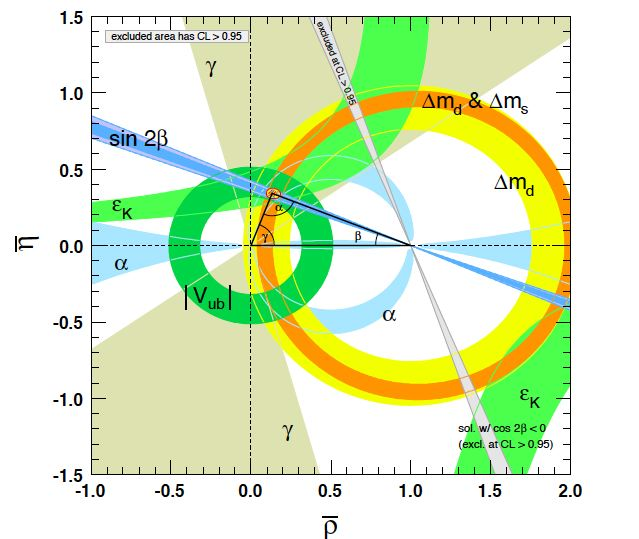
\includegraphics[width=9.5cm,height=6.0cm]{pics/CKMvincoli}
\end{figure}

$\gamma \equiv arg[-(V_{ud}V_{ub}^{*})/(V_{cd}V_{cb}^{*})]$ \newline

$\gamma$ can be studied using the interference between $b\rightarrow u$ and $b \rightarrow c$ transitions at tree level

\end{frame}

\begin{frame}
\frametitle{Why bother?}

$\gamma$ is the least well measured phase of the CKM triangle. Following results are obtained by averaging over several decay modes:

\begin{columns}

\column{.55\textwidth}
\begin{itemize}

\item LHCb: $\gamma = 73^{+9}_{-10}$

\item BaBar: $\gamma = 73^{+17}_{-16}$

\item Belle:  $\gamma = 68^{+15}_{-14}$

\end{itemize}


\column{.55\textwidth}
\begin{figure}
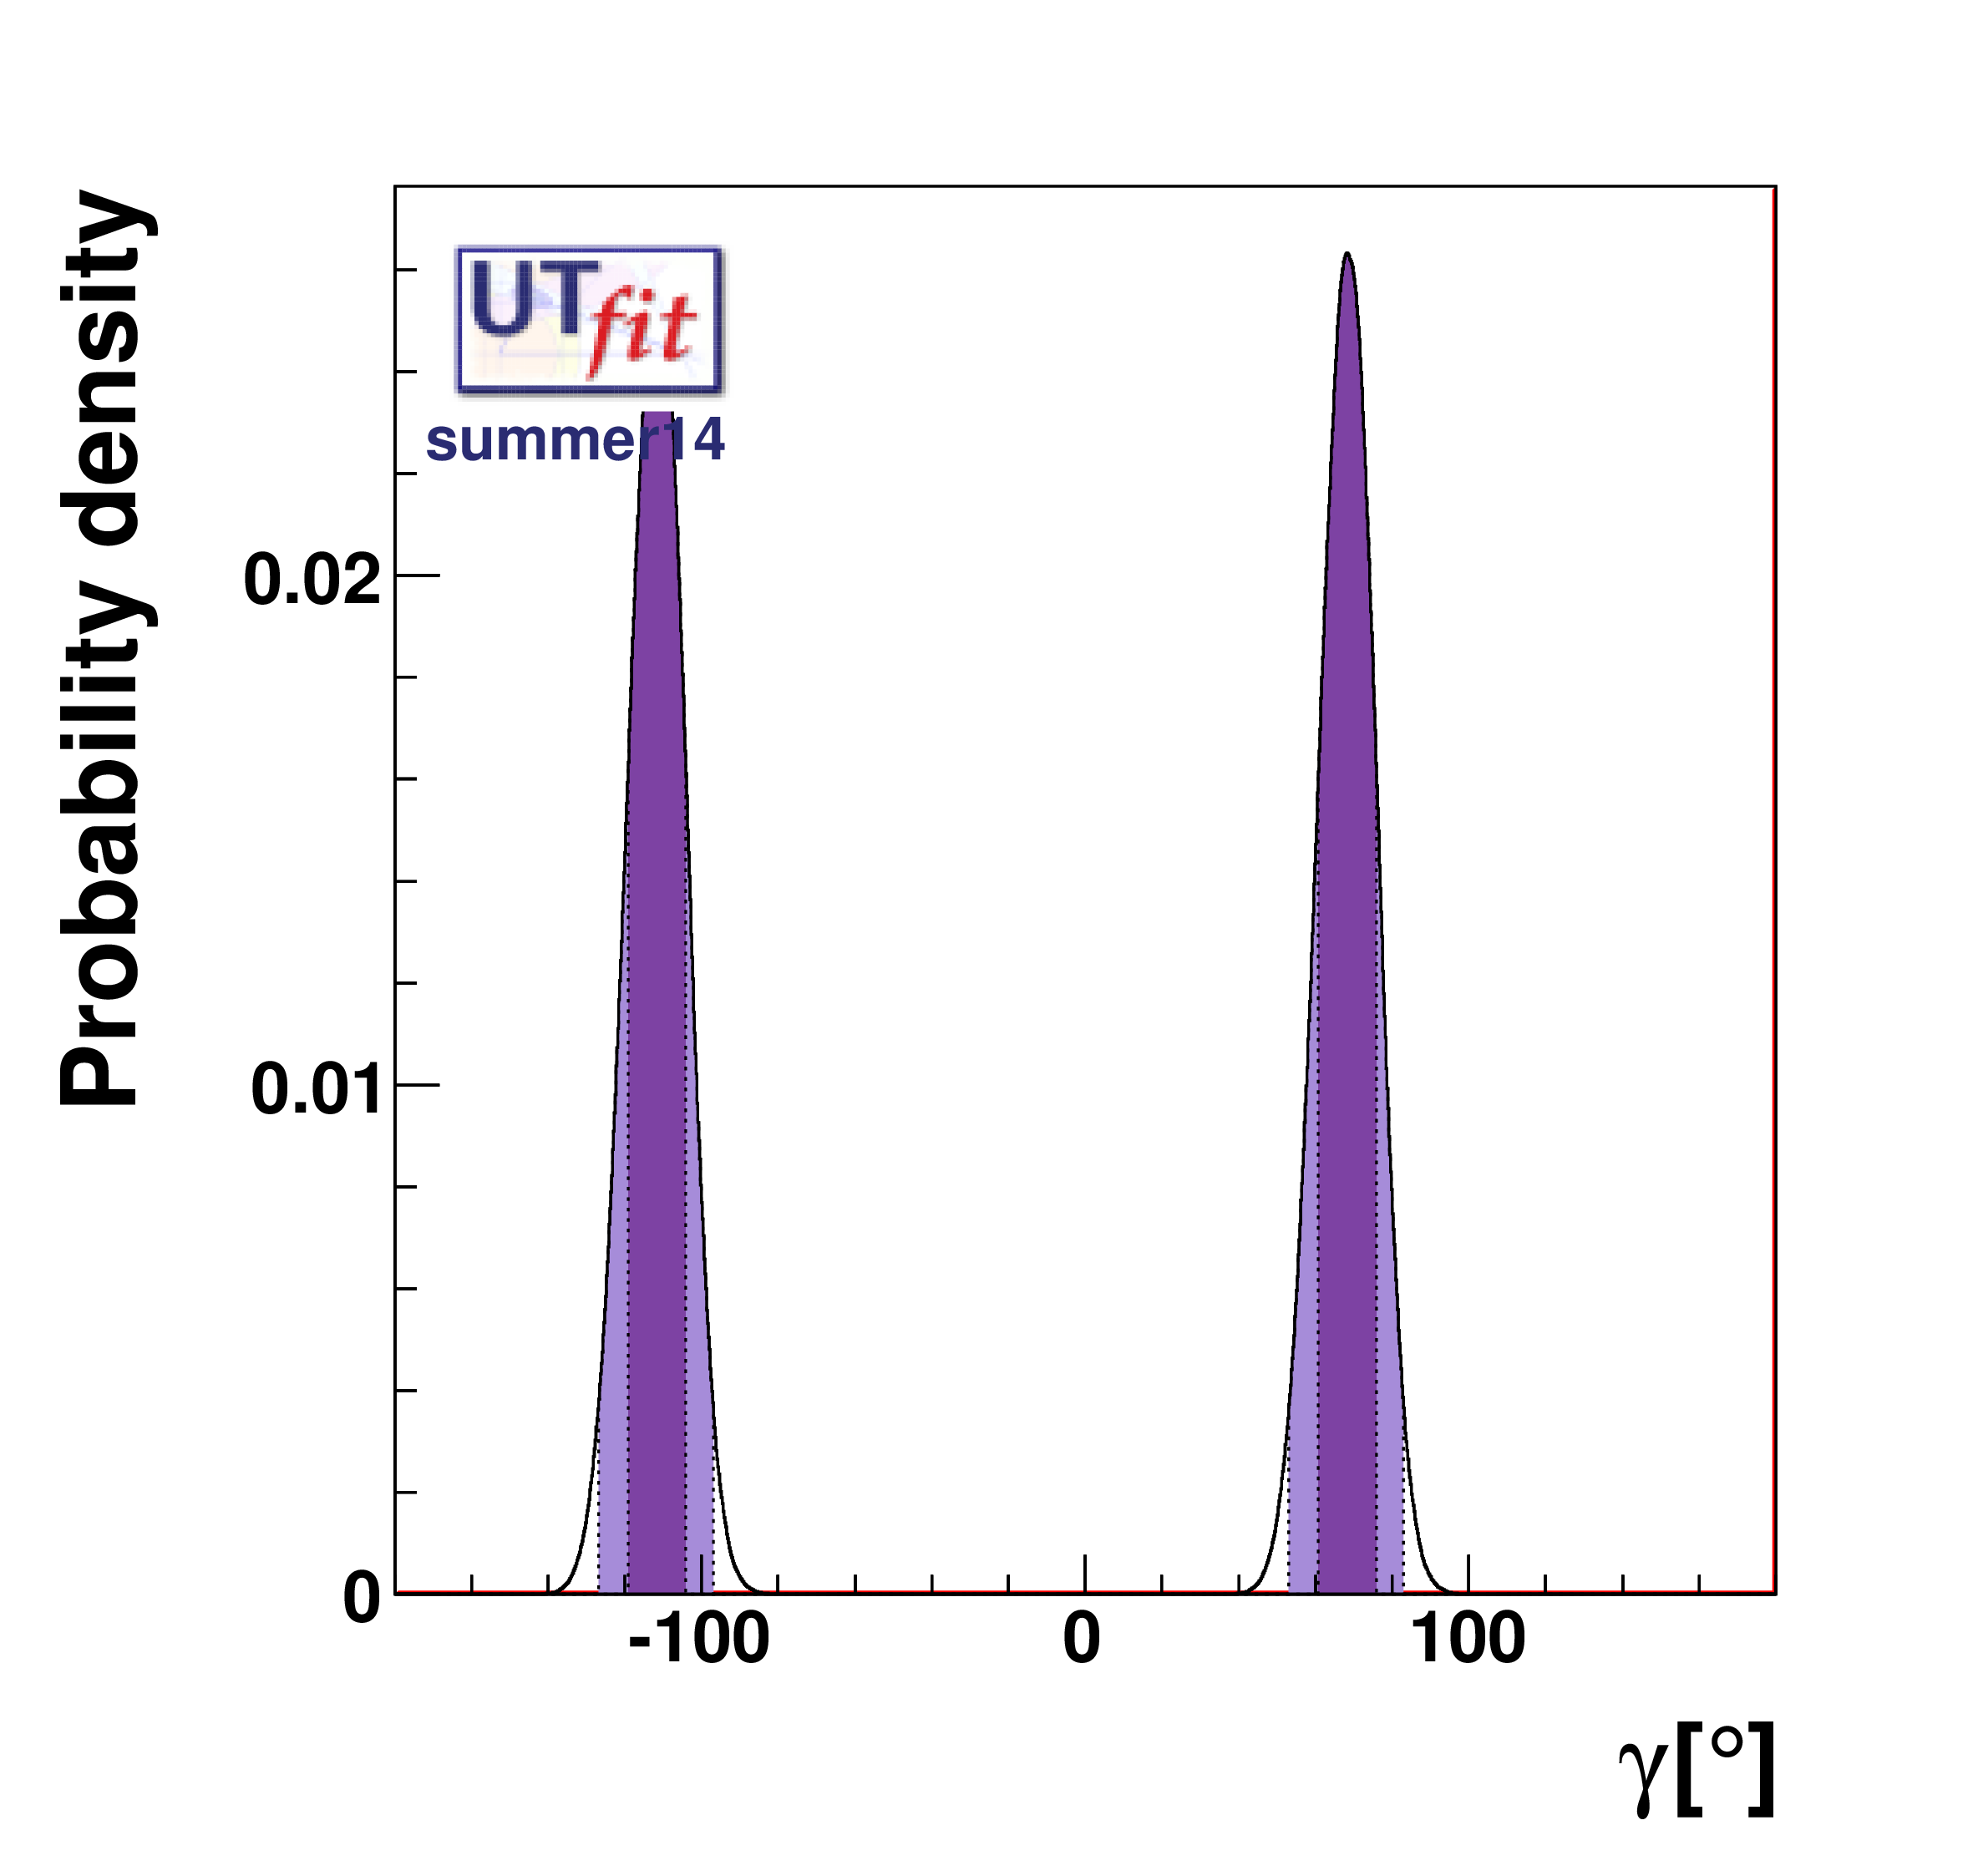
\includegraphics[width=6.0cm,height=4.0cm]{pics/summer14_gammaOUT_fullfit_gamma}
\end{figure}

\end{columns}

Precision of global fit $\approx 7\%$  v.s. the theory uncertainty of $<<1\%$  \newline \newline

$\rightarrow$ many unexplored channels left to improve the overall precision!

\end{frame}

\begin{frame}
\frametitle{And why this channel?}

\begin{figure}
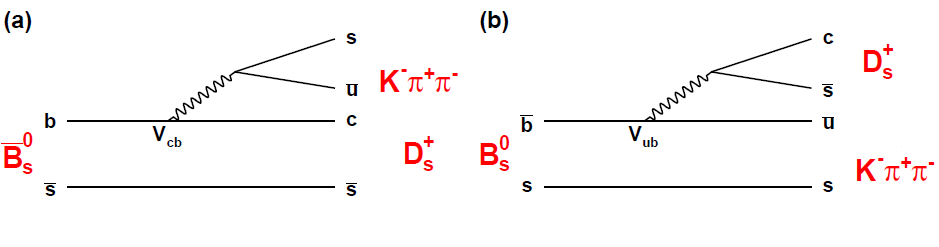
\includegraphics[width=11.0cm,height=4.5cm]{pics/FeynmannGraphs}
\end{figure}

interference between a) and b) with same final state via mixing \newline

complimentary to $\gamma$ determination in $B_{s}\rightarrow D_{s}K$ \newline

technically interesting application of time dependent amplitude analysis 

\end{frame}


\begin{frame}
\frametitle{What has been done}

First observation and BR mesurement done with 1 $fb^{-1}$ and $N_{D_{s}K\pi\pi} = 216 \pm 22$ in 2012 (LHCb-ANA-2012-076): 

\[\frac{\mathcal{B}(B_{s}\rightarrow D_{s}K\pi\pi)}{\mathcal{B}(B_{s}\rightarrow D_{s}\pi\pi\pi)} = (5.2\pm 0.5 \pm 0.3) \cdot 10^{-2}\]
 

\begin{figure}
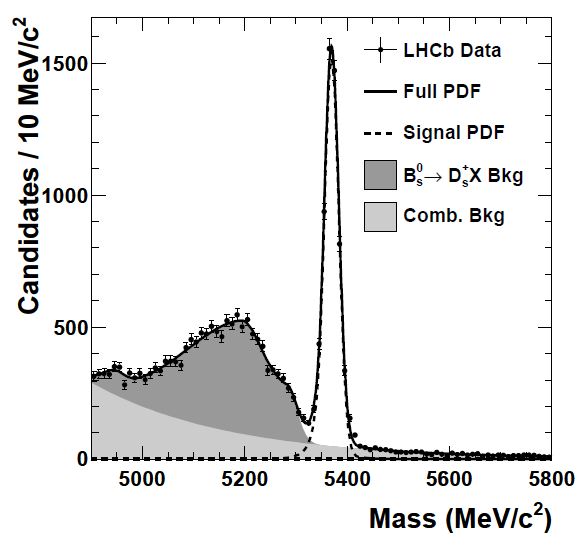
\includegraphics[width=5.5cm,height=3.7cm]{pics/BsDspipipi}
\subfigure{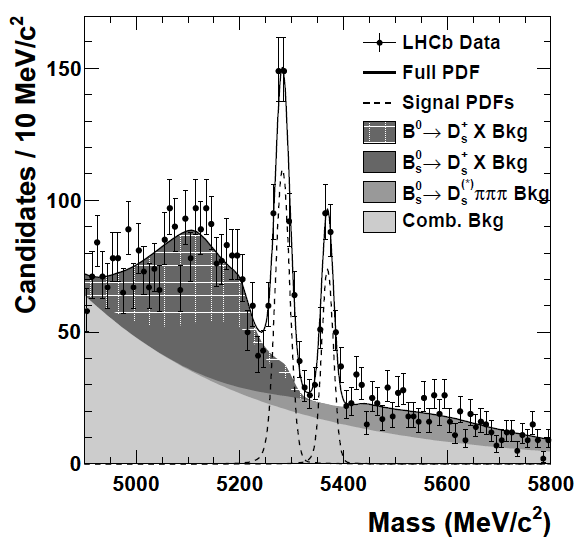
\includegraphics[width=5.5cm,height=3.7cm]{pics/BsDsKpipi}}
\caption{left: $D_{s}\pi\pi\pi$, right: $D_{s}K\pi\pi$}
\end{figure}


\end{frame}


\begin{frame}
\frametitle{Our plan}

We like to:
\begin{itemize}

\item redo the BR measurement with $3 fb^{-1}$ using $B_{s}\rightarrow D_{s}\pi\pi\pi$ as normalization channel

\item do a full time dependent daliz plot analysis to get strong phase difference and amplitude ratio across phase space to measure $\gamma$


\end{itemize} 

\bigskip

The analysis follows principle of $\gamma$ measurement in $B_{s}\rightarrow D_{s}K$, but with additional pion pair the dalitz analysis is necessary

\end{frame}


\begin{frame}
\frametitle{Stripping}

We produced Data and MC ntuples for 2011 and 2012:

\begin{tabular}{l|l|l}
Year & Channel & Stripping \\ \hline
2011 & $D_{s}K\pi\pi$ & B02DKPiPiD2HHHPIDBeauty2Charm, S21 \\
2012 & $D_{s}K\pi\pi$ & B02DKPiPiD2HHHPIDBeauty2Charm, S21\\
2011 & $D_{s}\pi\pi\pi$ & B02DPiPiPiD2HHHPIDBeauty2Charm, S21 \\
2012 & $D_{s}\pi\pi\pi$ & B02DPiPiPiD2HHHPIDBeauty2Charm, S21\\
\end{tabular} \newline

Additionally, we produced $B_{s}\rightarrow D_{s}^{*}X$ MC samples to constrain peaking background (see later) \newline

The plan is to use all possible final states, with $D_{s}\rightarrow KK\pi,K\pi\pi,\pi\pi\pi$ \newline

We expect O(1k) signal events

\end{frame}


\begin{frame}
\frametitle{Stripping Selection}
Stripping and (pre-)selection cuts include:

\begin{itemize}

\item all tracks: $p > 1$ $GeV$ , $p_{t} > 100$ $MeV$, $track\chi^{2}/ndof < 3$ and $IP\chi^{2} > 4$ 

\item $D_{s}$ daughter: $\Sigma p_{t} > 1.8$ $GeV$, max DOCA 0.5mm and $M_{KK\pi}$ within 100 $MeV$ of $M_{D_{s}}$  

\item $D_{s}$: $Vertex\chi^{2}/ndof < 10$ and min $FD\chi^{2} > 36$ 

\item $B_{s}$: $DIRA > 0.99$, min $IP\chi^{2} > 20$, $FD\chi^{2} > 100$ and vertex fit $\chi^{2}/ndof < 8$

\item loose PID requirements on the final state \\ kaons ($\Delta LL(K - \pi) > -5$) and pions ($\Delta LL(K - \pi) < 10$)

\end{itemize}

\end{frame}

\begin{frame}

\frametitle{Physical Background}

In addition to the previous cuts, we veto some specific backgrounds such as:

\begin{itemize}

\item $B_{s}\rightarrow D_{s}D_{s}$: \newline
 $|M(K\pi\pi) - m_{D_{s}}| > 20$ $MeV$

\item $B^{0}\rightarrow D^{+}(\rightarrow K\pi\pi)K\pi\pi$: \newline
 possible with single miss-ID. Vetoed by changing $K^{+}\rightarrow\pi^{+}$ mass hypothesis and check $|M(K^{+}\pi^{-}\pi^{+}) - m_{D^{+}}| > 20$ $MeV$ \newline
$||$ $\Delta LL(K - \pi) > 10$ for the $K^{+}$

\item $\Lambda_{b}^{0}\rightarrow \Lambda_{c}^{+}(\rightarrow Kp\pi)K\pi\pi$: \newline
 possible with single miss-ID. Vetoed by assigning $K^{+}\rightarrow p$ and check $|M(pK^{-}\pi^{+}) - m_{\Lambda_{c}^{+}}| > 15$ $MeV$ \newline
$||$ $\Delta LL(K - p) > 0$ for the $K^{+}$

\end{itemize}

\end{frame}

%
%\begin{frame}
%\frametitle{First plots}
%
%After the preselection of candidates we get (only $D_{s}\rightarrow KK\pi$):
%
 %\begin{figure}
%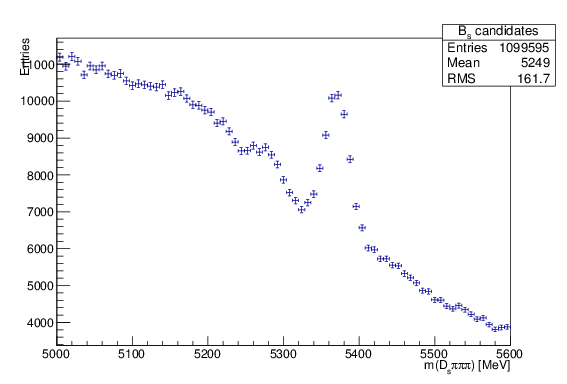
\includegraphics[width=5.5cm,height=3.7cm]{pics/mass_Bs_preSel_12Data_3pi.png}
%\subfigure{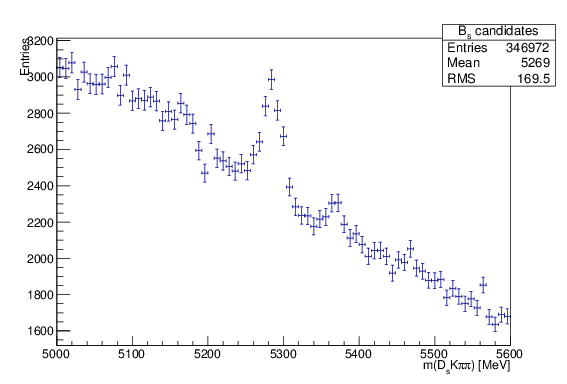
\includegraphics[width=5.5cm,height=3.7cm]{pics/mass_Bs_preSel_12Data.png}}
%\caption{invariant mass of left: $B_{s}\rightarrow D_{s}\pi\pi\pi$ candidates , right: $B_{s}\rightarrow D_{s}K\pi\pi$ candidates}
%\end{figure}
%
%
%$\rightarrow$ further selection via multivariate method
%
%\end{frame}


\begin{frame}
\frametitle{TMVA}

We take the upper mass sideband of $B_{s}$ data candidates as background and MC signal events \newline

Variables used for BDTG training, with $X_{s} = (K\pi\pi)$:

\begin{itemize}

\item $log(min(IP\chi^{2}))$ and $log(max(IP\chi^{2}))$ of $D_{s}$ daughters

\item $log(min(IP\chi^{2}))$ and $log(max(IP\chi^{2}))$ of $X_{s}$ daughters

\item $log((IP\chi^{2}))$ of $X_{s}$

\item $log((IP\chi^{2}))$ of $B_{s}$

\item FD significance of $B_{s}$ and $D_{s}$

\item $log(min(p_{t}))$ of $D_{s}$ and $X_{s}$ daughters

\item $B_{s}$ vertex fit $\chi^{2}$ 

\item $max(track\chi^{2})$

\item Cone $p_{t}$ asymmetry of all tracks 

\item max(track-ghostProb)

\end{itemize}

\end{frame}



\begin{frame}
\frametitle{BDTG output}

\begin{figure}
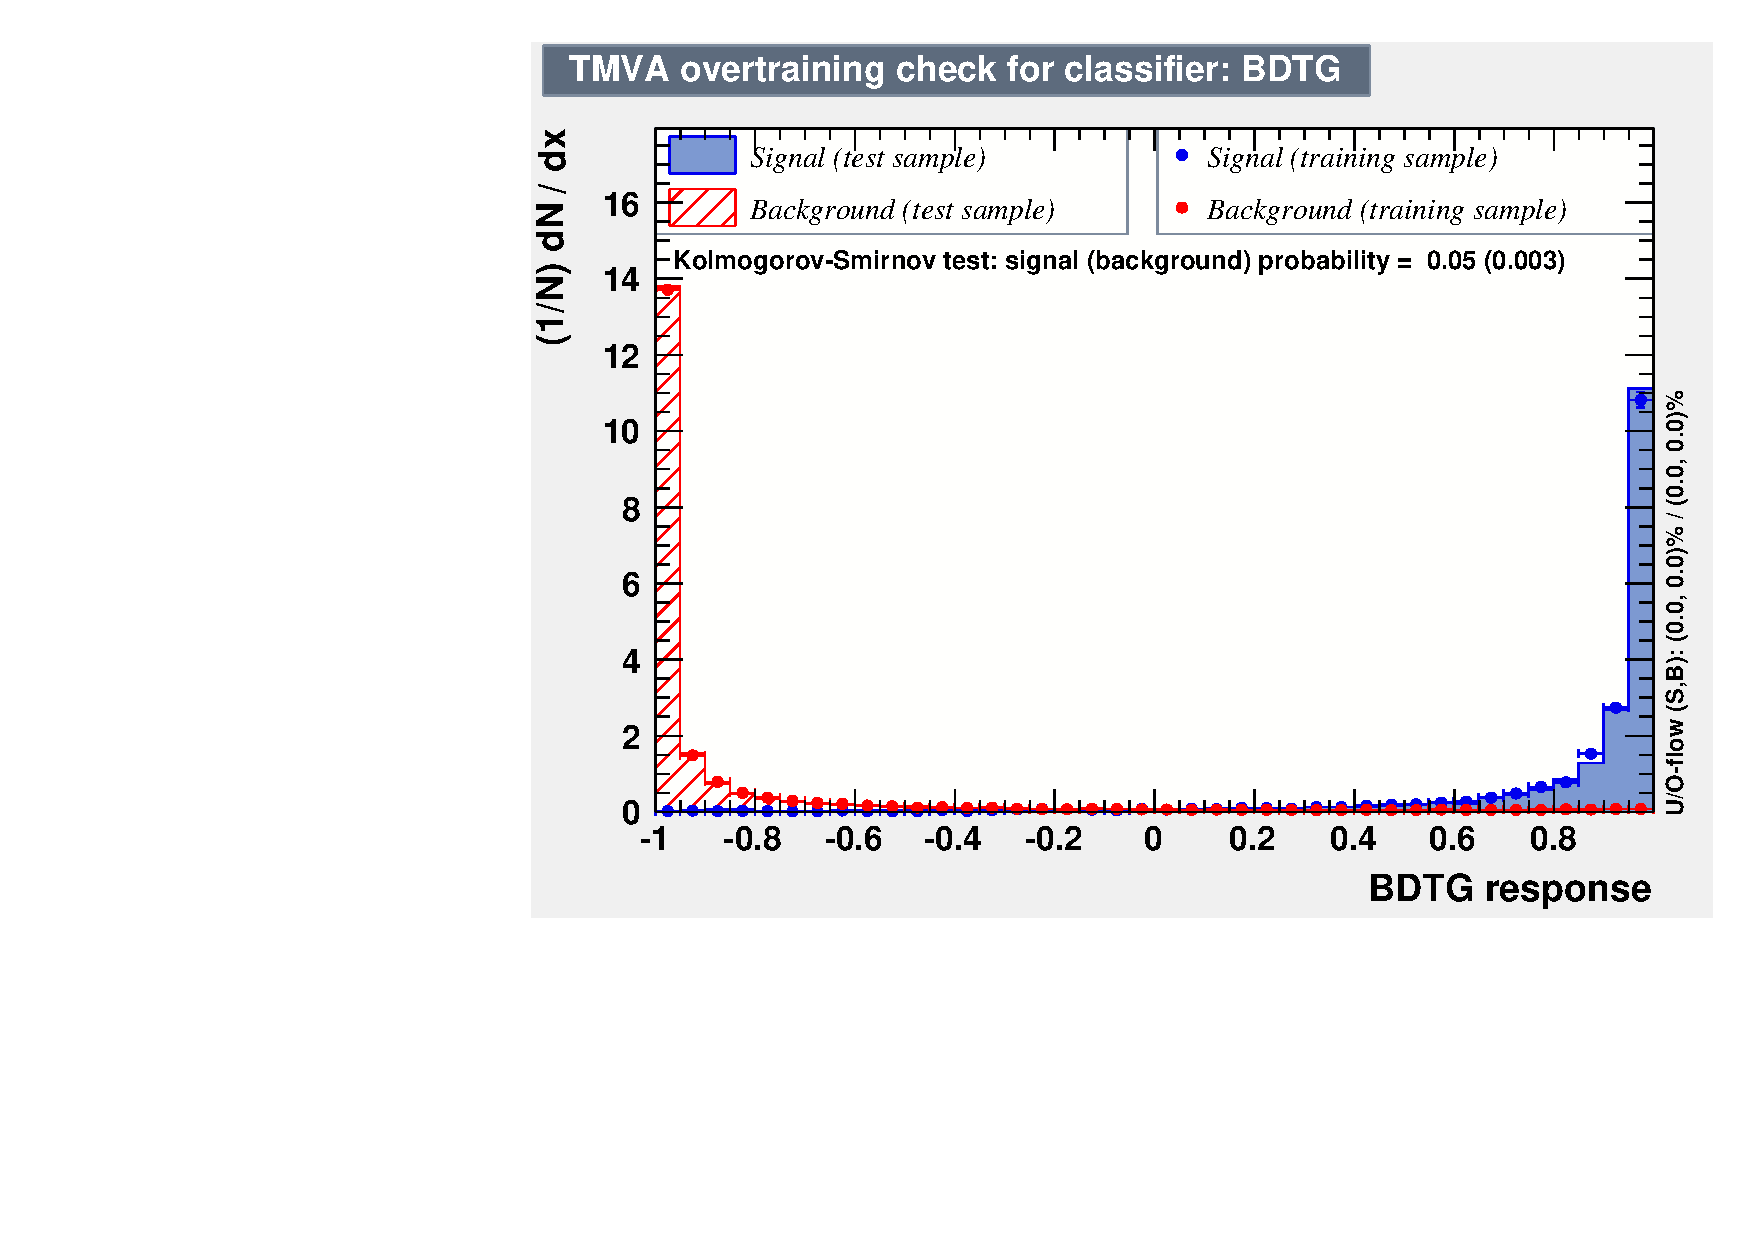
\includegraphics[width=5.5cm,height=4.0cm]{pics/BDT_Response_BDTG}
\subfigure{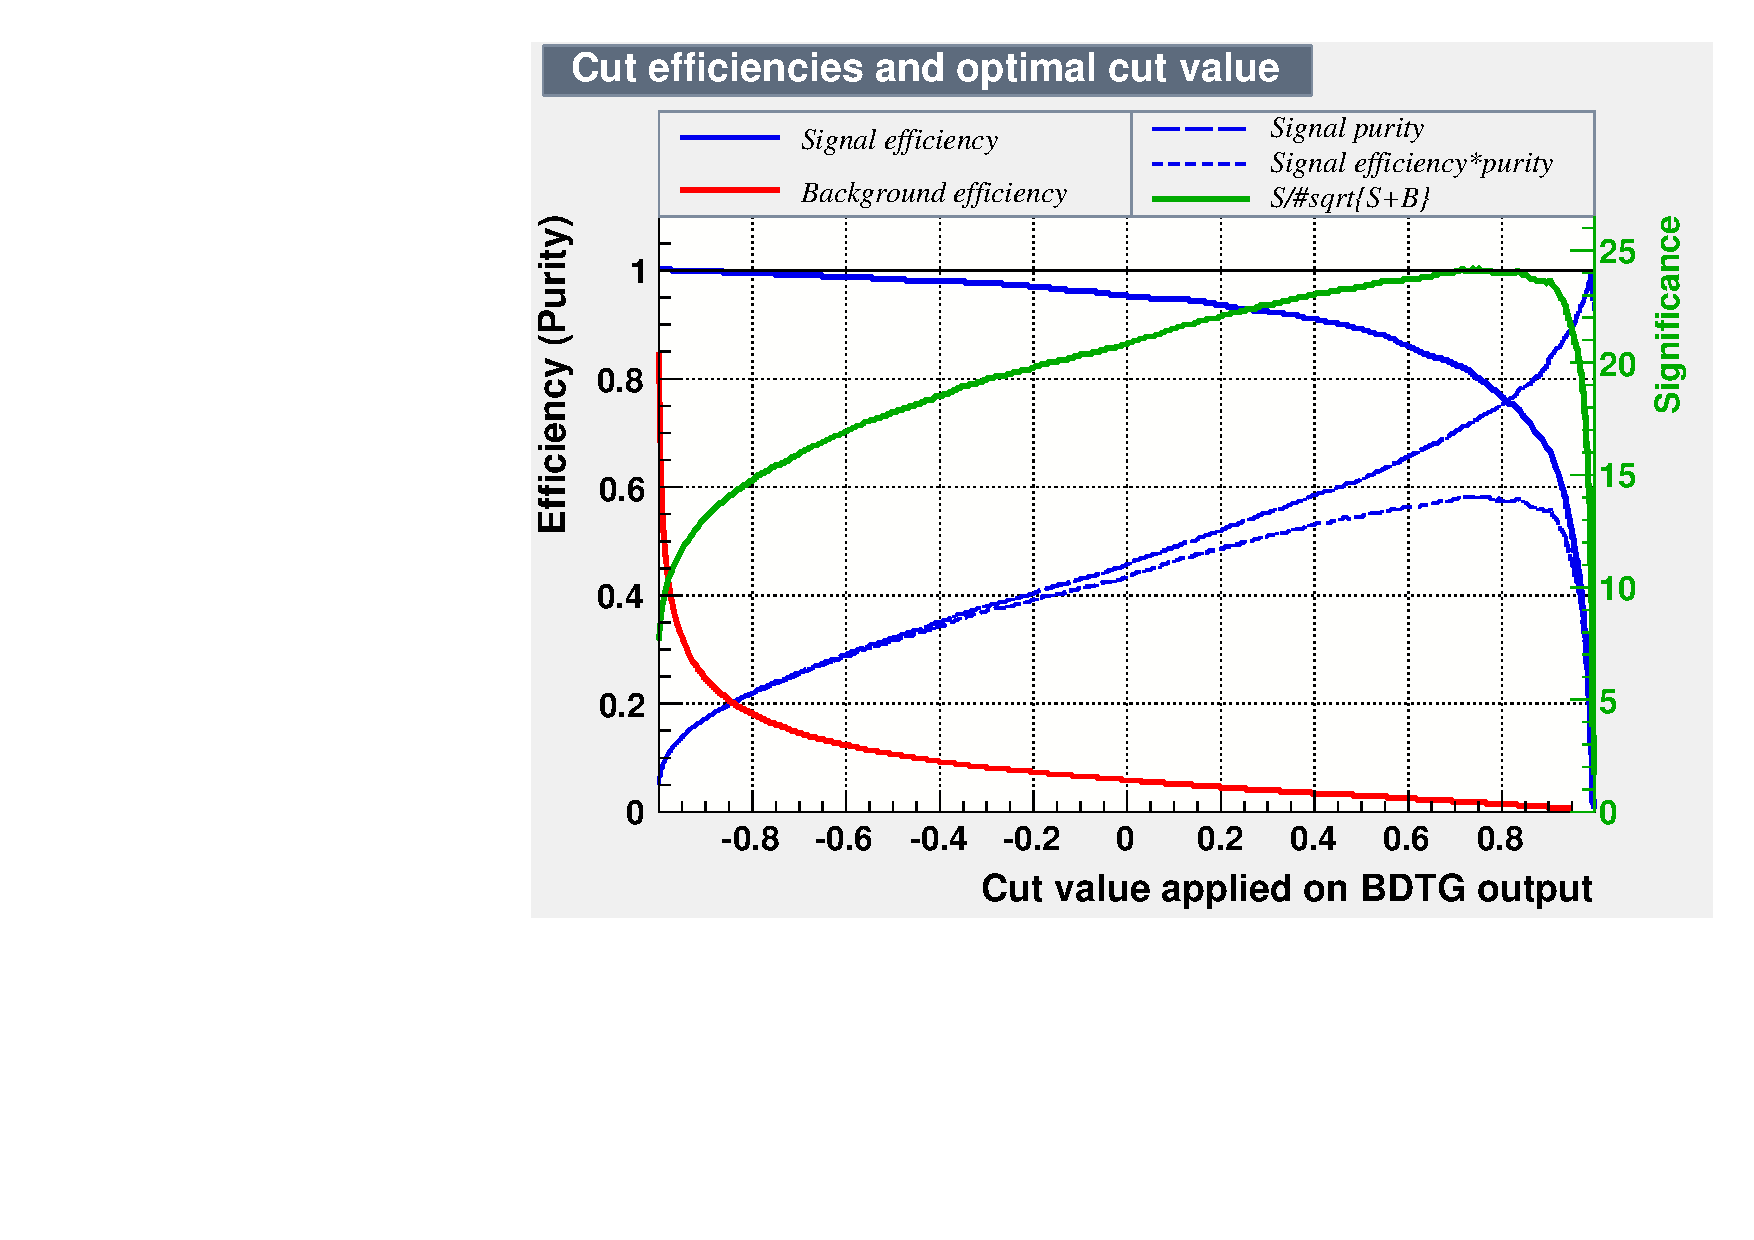
\includegraphics[width=5.5cm,height=4.0cm]{pics/BDT_Effizienz_BDTG}}
\caption{left: BDTG response, right: BDTG efficiency curves}
\end{figure}

We optimize our response cut using a massfit in the $B_{s}\rightarrow D_{s}\pi\pi\pi$ channel after pre-selection and scale the obtained value for S with the PDG BR and relative efficiency to $B_{s}\rightarrow D_{s}K\pi\pi$   


\end{frame}

\begin{frame}
\frametitle{Background Shape for normalization channel}

 %Physical background shape for $B_{s}\rightarrow D_{s}\pi\pi\pi$ (from MC):

 \begin{figure}
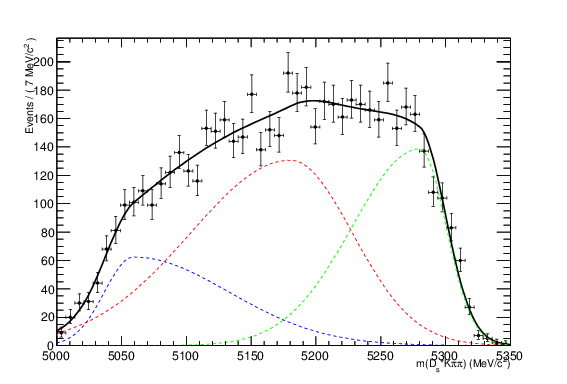
\includegraphics[width=8.0cm,height=5.5cm]{pics/Bs2Dsstartpipipi.png}
\caption{partially reconstructed $B_{s}\rightarrow D_{s}^{*}\pi\pi\pi$}
\end{figure}

\end{frame}

\begin{frame}
\frametitle{Background Shapes for signal channel}

 %Physical background shapes for $B_{s}\rightarrow D_{s}K\pi\pi$ (from MC):

\begin{figure}
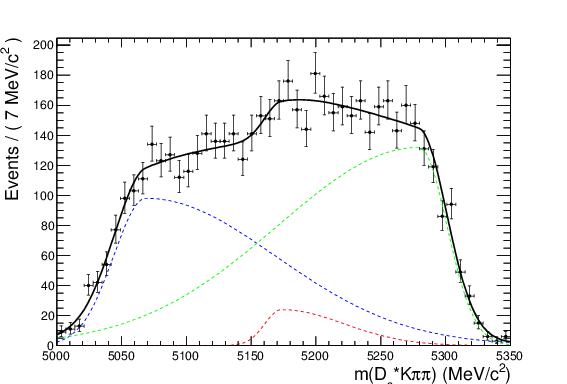
\includegraphics[width=4.5cm,height=2.0cm]{pics/Bs2DsstartKpipi.png}
\subfigure{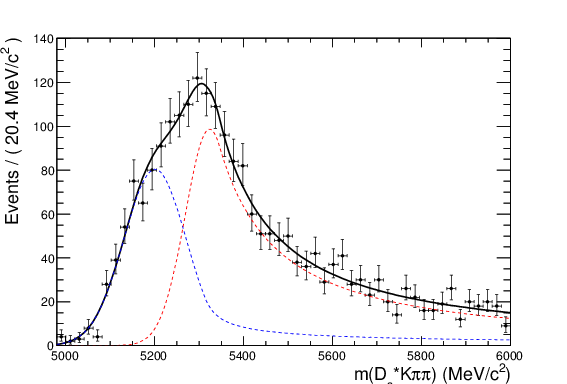
\includegraphics[width=4.5cm,height=2.0cm]{pics/Bs2Dsstarpipipi_as_DsKpipi.png}}\\
\subfigure{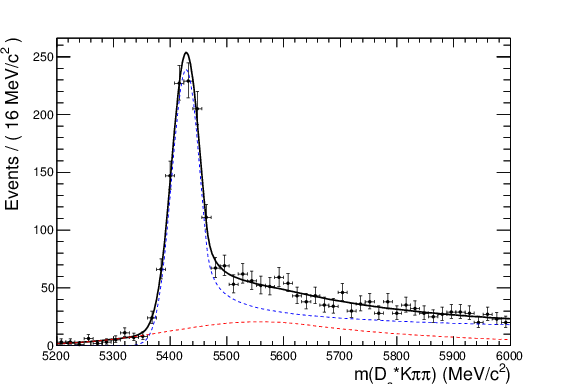
\includegraphics[width=4.5cm,height=2.0cm]{pics/Bs2Dspipipi_as_DsKpipi}}
\caption{top left: partially reconstructed $B_{s}\rightarrow D_{s}^{*}K\pi\pi$,\newline top right: $B_{s}\rightarrow D_{s}^{*}\pi\pi\pi$ miss-id, bottom: $B_{s}\rightarrow D_{s}\pi\pi\pi$ miss-id}
\end{figure}

\small

\textcolor{red}{Dangerous}: $B_{s}\rightarrow D_{s}^{(*)}\pi\pi\pi$ miss-id peaks in signal region $\rightarrow$ control contributions using PID calib
  
\normalsize

\end{frame}

\begin{frame}
\frametitle{Mass fits in normalization channel}

\begin{figure}
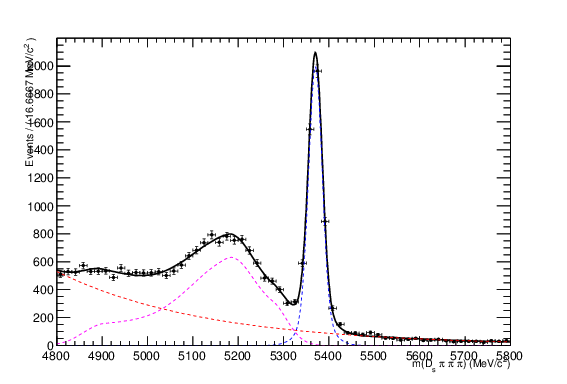
\includegraphics[width=5.4cm,height=3.8cm]{pics/3pi_BmassFit_11}
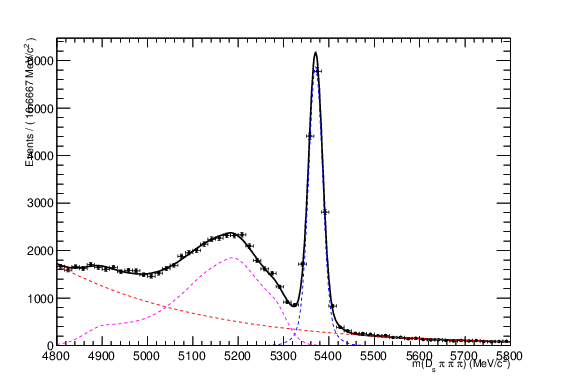
\includegraphics[width=5.4cm,height=3.8cm]{pics/3pi_BmassFit_12}\\
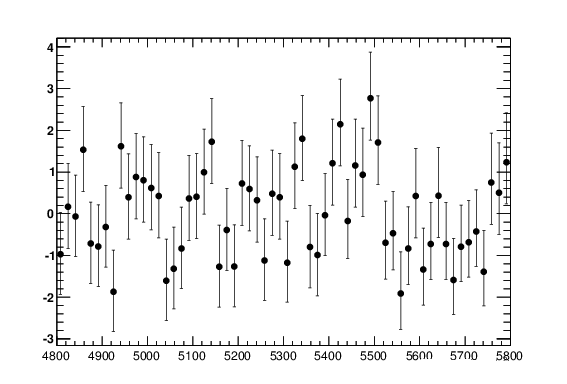
\includegraphics[width=5.4cm,height=1.5cm]{pics/3pi_pull_11}
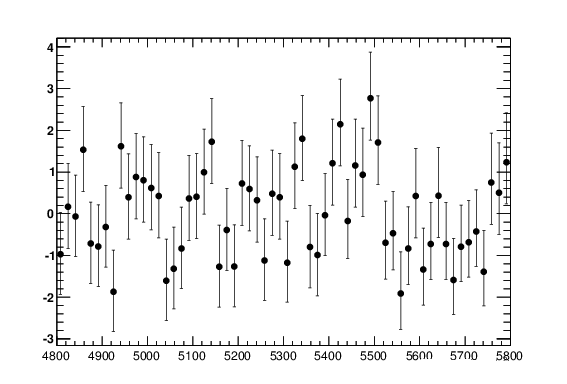
\includegraphics[width=5.4cm,height=1.5cm]{pics/3pi_pull_11}
\caption{Invariant mass distribution for $B_{s}\rightarrow D_{s}\pi\pi\pi$ candidates for (left) 2011 and (right) 2012}
\end{figure}

%$PDF(m_{B};\vec{\lambda}) = N_{Sig}\cdot DG(m_{B};\overline{m},\sigma) + N_{PhysBG}\cdot 3Bif.Gauss(m_{B};\overline{m},\sigma_{L},\sigma_{R}) + N_{comb}\cdot exp(m_{B};\alpha)$ \newline


\end{frame}

\begin{frame}
\frametitle{Mass fits in signal channel}

\begin{figure}
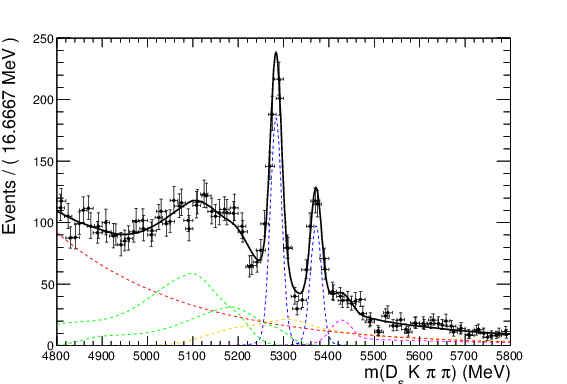
\includegraphics[width=5.4cm,height=3.8cm]{pics/BmassFit_11}
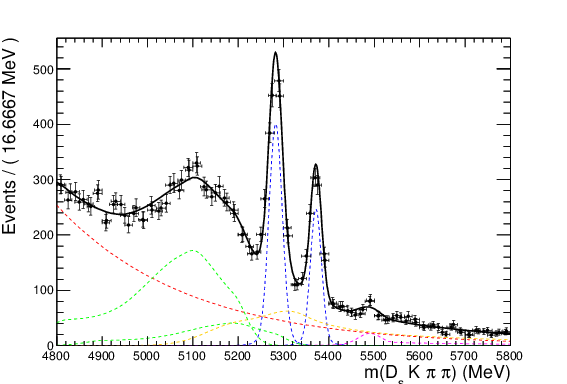
\includegraphics[width=5.4cm,height=3.8cm]{pics/BmassFit_12}\\
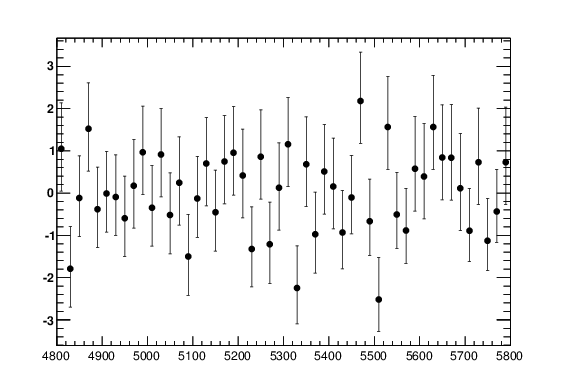
\includegraphics[width=5.4cm,height=1.5cm]{pics/pull_11}
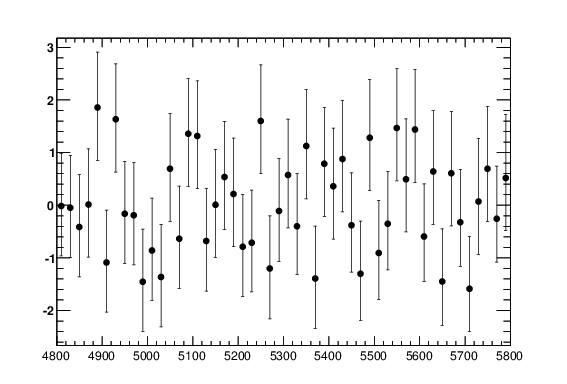
\includegraphics[width=5.4cm,height=1.5cm]{pics/pull_12}
\caption{Invariant mass distribution for $B_{s}\rightarrow D_{s} K\pi\pi$ candidates for (left) 2011 and (right) 2012}
\end{figure}

%$PDF(m_{B};\vec{\lambda}) = N_{B^{0}}\cdot DG(m_{B^{0}};\overline{m},\sigma) + N_{Sig}\cdot DG(m_{B_{s}};\overline{m},\sigma) + N_{PhysBG}\cdot (3Bif.Gauss(m_{B};\overline{m},\sigma_{L},\sigma_{R}) + 2DCB(miss-id)) + N_{comb}\cdot exp(m_{B};\alpha)$ \newline

\end{frame}

\begin{frame}
\frametitle{Yields (not final, only $D_{s}\rightarrow K K \pi$)}

for the normalization channel we extract:

\begin{itemize}

\item 2011: $N_{B_{s}\rightarrow D_{s}\pi\pi\pi} = 4927 \pm 85$ \newline
\item 2012: $N_{B_{s}\rightarrow D_{s}\pi\pi\pi} = 14566 \pm 141$ \newline

\end{itemize}


and for the signal channel:

\begin{itemize}

\item 2011: $N_{B_{s}\rightarrow D_{s}K\pi\pi} = 201 \pm 21$ \newline
\item 2012: $N_{B_{s}\rightarrow D_{s}K\pi\pi} = 474 \pm 32$ \newline

\end{itemize}

\end{frame}



\begin{frame}
\frametitle{MC-Data comparison 1}

using the shown massfit we can get signal sWeights for data \newline

$\rightarrow$ compare distributions of sWeighted data and signal MC

\begin{figure}
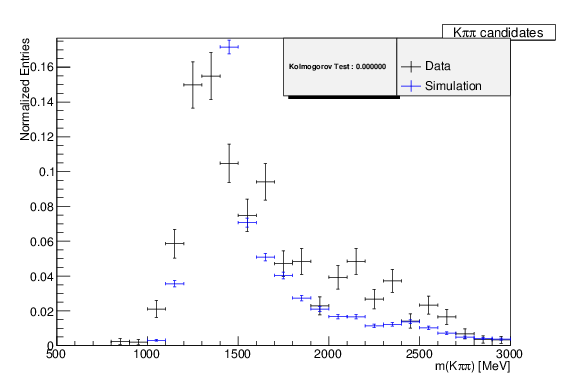
\includegraphics[width=5.5cm,height=4.0cm]{pics/m_Kpipi_comp.png}
\subfigure{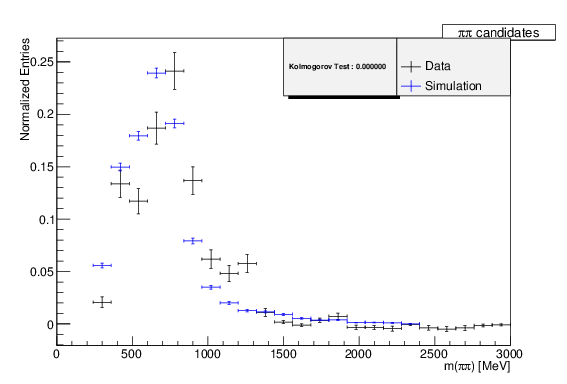
\includegraphics[width=5.5cm,height=4.0cm]{pics/m_pipi_comp.png}}
\end{figure}

\end{frame}

\begin{frame}
\frametitle{MC-Data comparison 2}

\begin{figure}
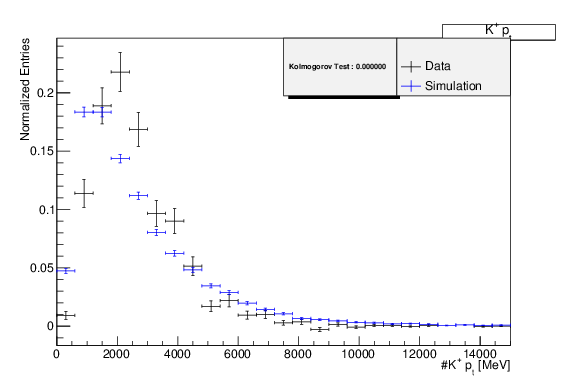
\includegraphics[width=5.5cm,height=4.0cm]{pics/p_KPlus_comp.png}
\subfigure{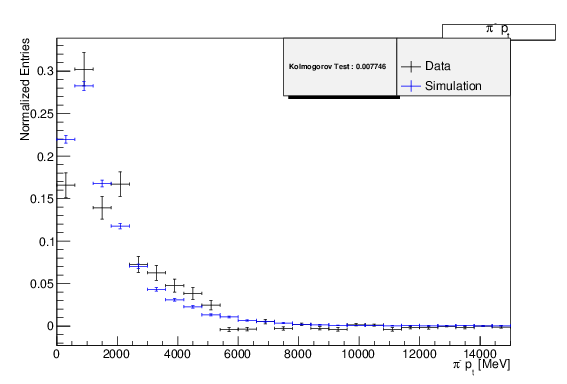
\includegraphics[width=5.5cm,height=4.0cm]{pics/p_piMinus_comp.png}}
\end{figure}

\end{frame}

\begin{frame}
\frametitle{MC-Data comparison 3}

\begin{figure}
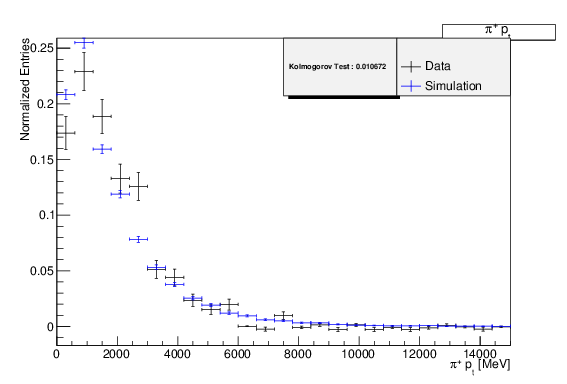
\includegraphics[width=5.5cm,height=4.0cm]{pics/p_piPlus_comp.png}
\end{figure}

\end{frame}

\begin{frame}
\frametitle{MC-Data comparison 4}

\begin{figure}
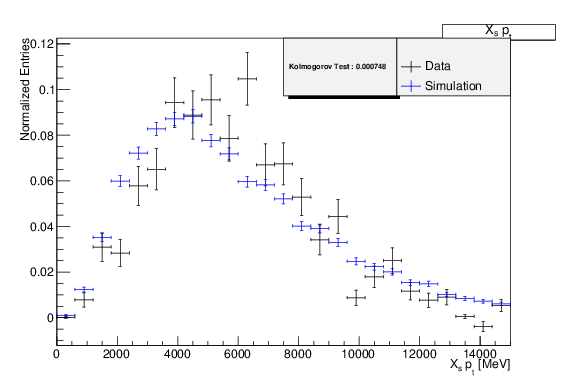
\includegraphics[width=5.5cm,height=4.0cm]{pics/pt_Xs_comp.png}
\subfigure{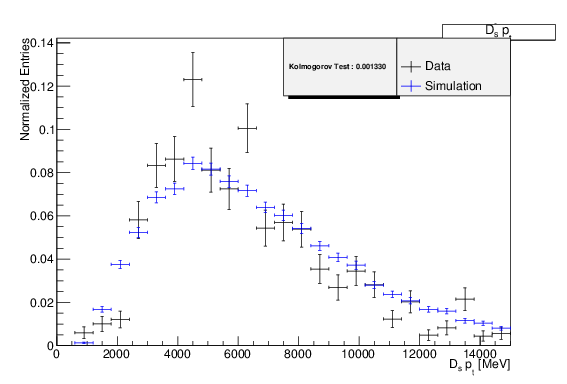
\includegraphics[width=5.5cm,height=4.0cm]{pics/pt_Ds_comp.png}}
\end{figure}

\end{frame}

\begin{frame}
\frametitle{MC-Data comparison 5}

\begin{figure}
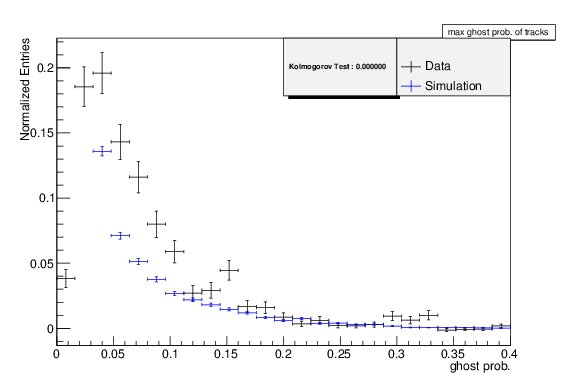
\includegraphics[width=5.5cm,height=4.0cm]{pics/max_ghostProb_comp.png}
\subfigure{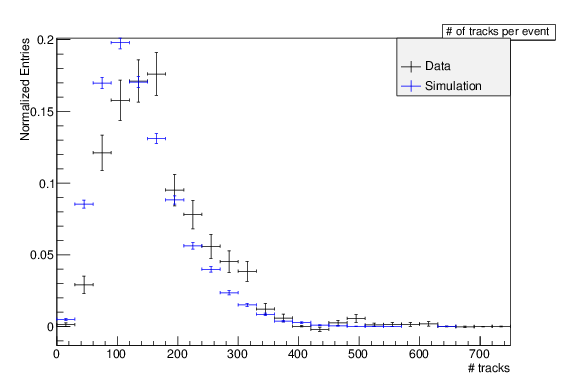
\includegraphics[width=5.5cm,height=4.0cm]{pics/nTracks_comp.png}}
\end{figure}

\end{frame}

\begin{frame}
\frametitle{Outlook}

Next steps:

\begin{itemize}

\item check efficiencies between normalization and signal channel

\item make sure the PIDCalib samples are correct (some problems were reported): results crucial to fix yields of physical background which affects signal yield directly 

\item finalize the BR measurement: could be finished very quick, but depends strongly on my/our hardware occupancy (atm $99\%$ since November Testbeam) 

\item write ANA Note
			
\item move on to amplitude analysis 

%\item add $D_{s}\rightarrow \pi\pi\pi$ and $D_{s}\rightarrow K \pi \pi$ final states (began to look into this). Remember: \newline
	%		$BR(D_{s}\rightarrow K\pi\pi) \approx \frac{1}{10} \cdot BR(D_{s}\rightarrow KK\pi)$ \newline
	%		$BR(D_{s}\rightarrow \pi\pi\pi) \approx \frac{1}{5} \cdot BR(D_{s}\rightarrow KK\pi)$

\end{itemize}

\end{frame}

\appendix 
\addtocounter{framenumber}{-1} 

\begin{frame}
\thispagestyle{empty}
\bfseries\Huge

\begin{center}
BACKUP
\end{center}

\normalfont

\end{frame}

\begin{frame}
\frametitle{BDT Input 1}

\begin{figure}
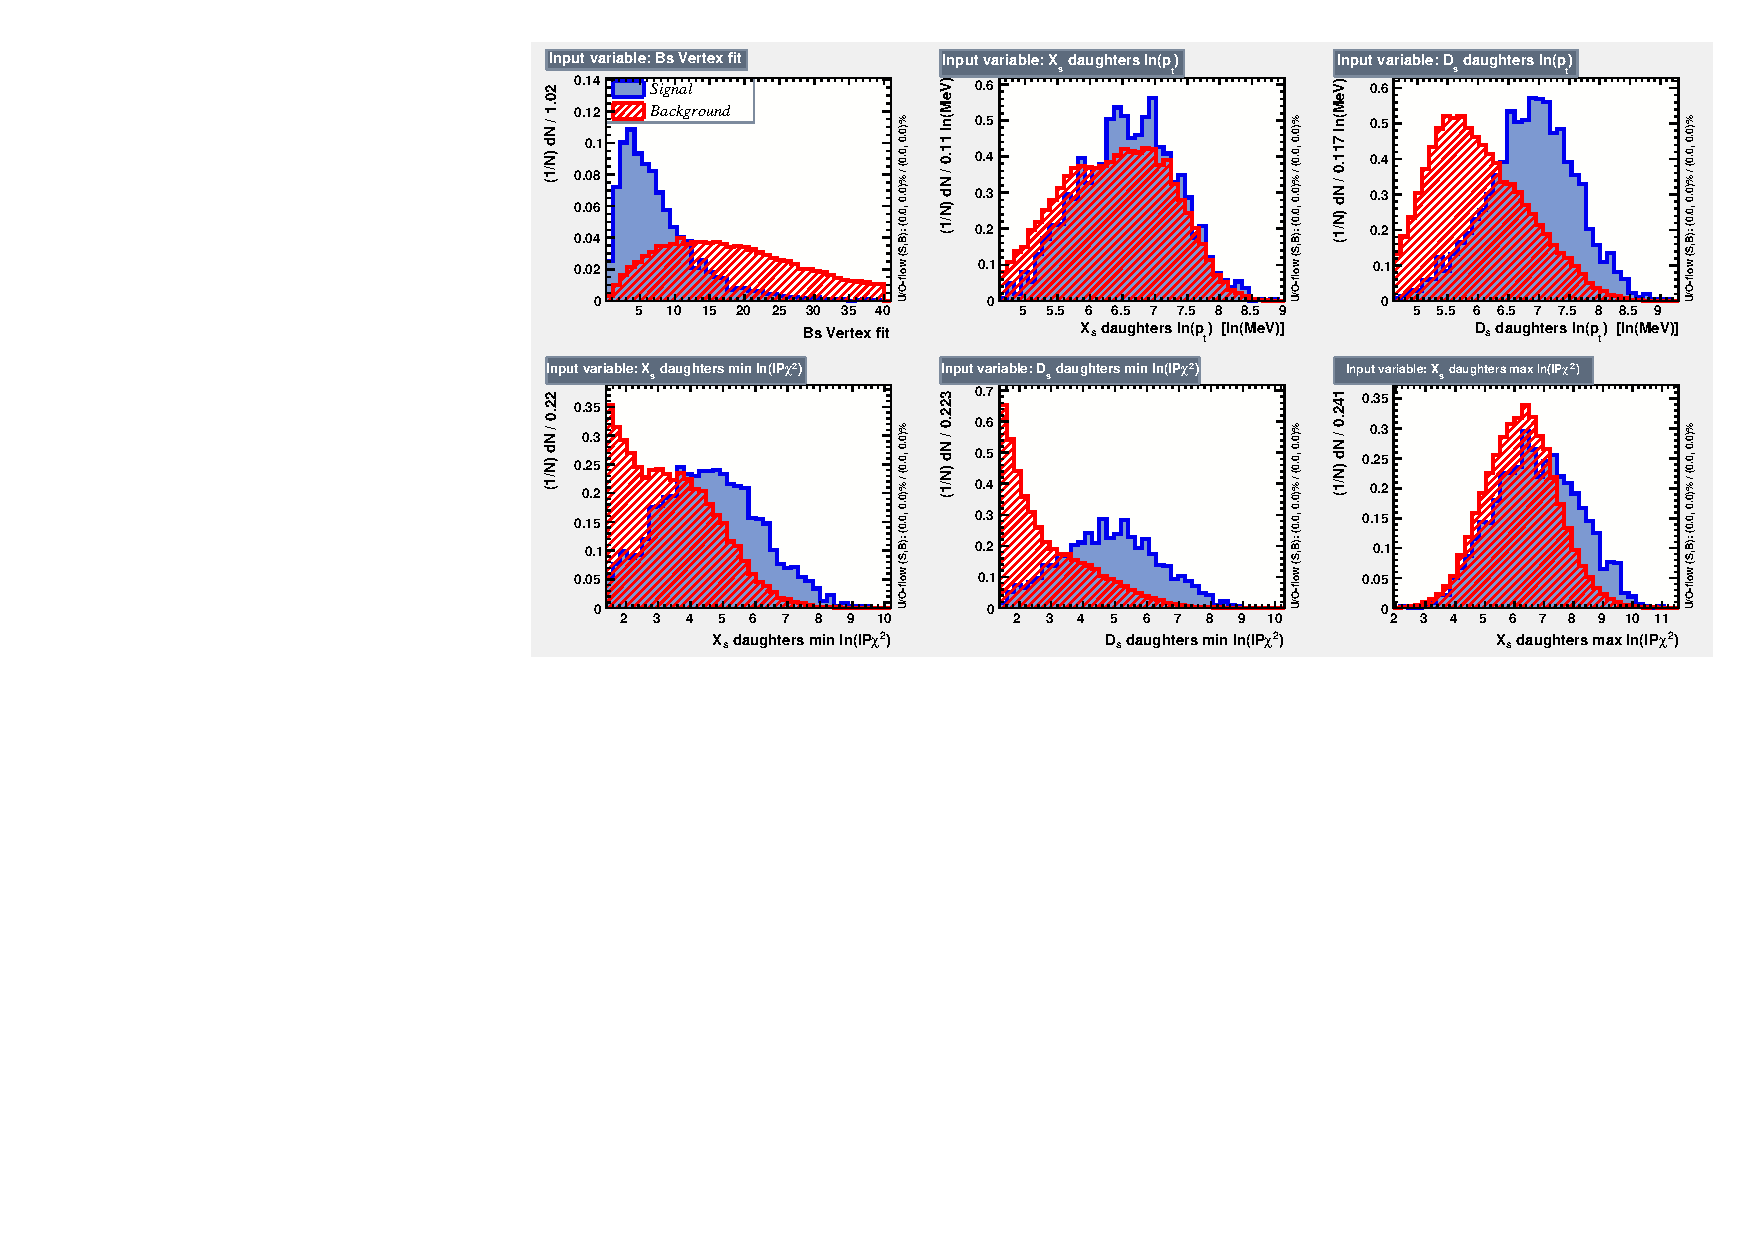
\includegraphics[width=10.0cm,height=5.5cm]{pics/BDT_Input_12_1}
\end{figure}

\end{frame}
\begin{frame}
\frametitle{BDT Input 2}

\begin{figure}
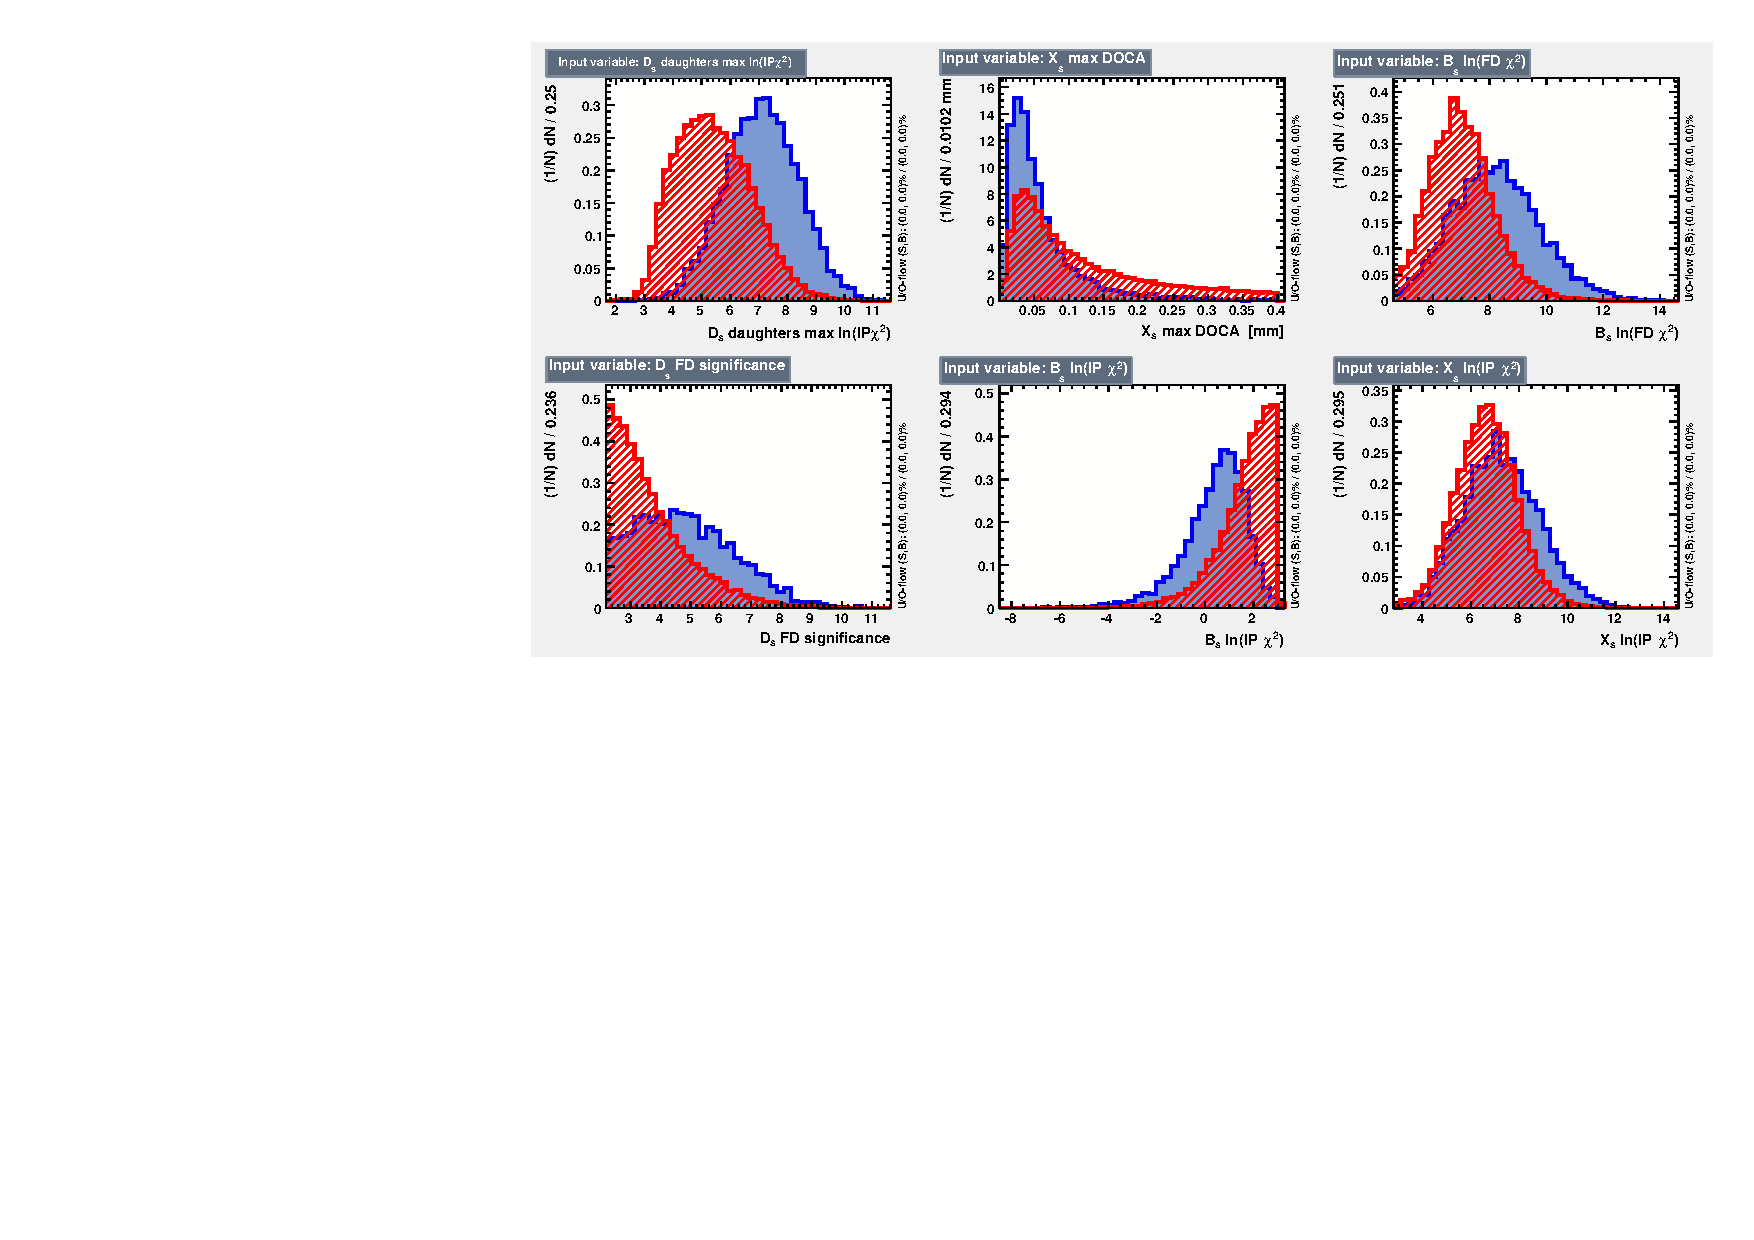
\includegraphics[width=10.0cm,height=5.5cm]{pics/BD_Input_12_2}
\end{figure}

\end{frame}

\begin{frame}
\frametitle{BDT Input 3}

\begin{figure}
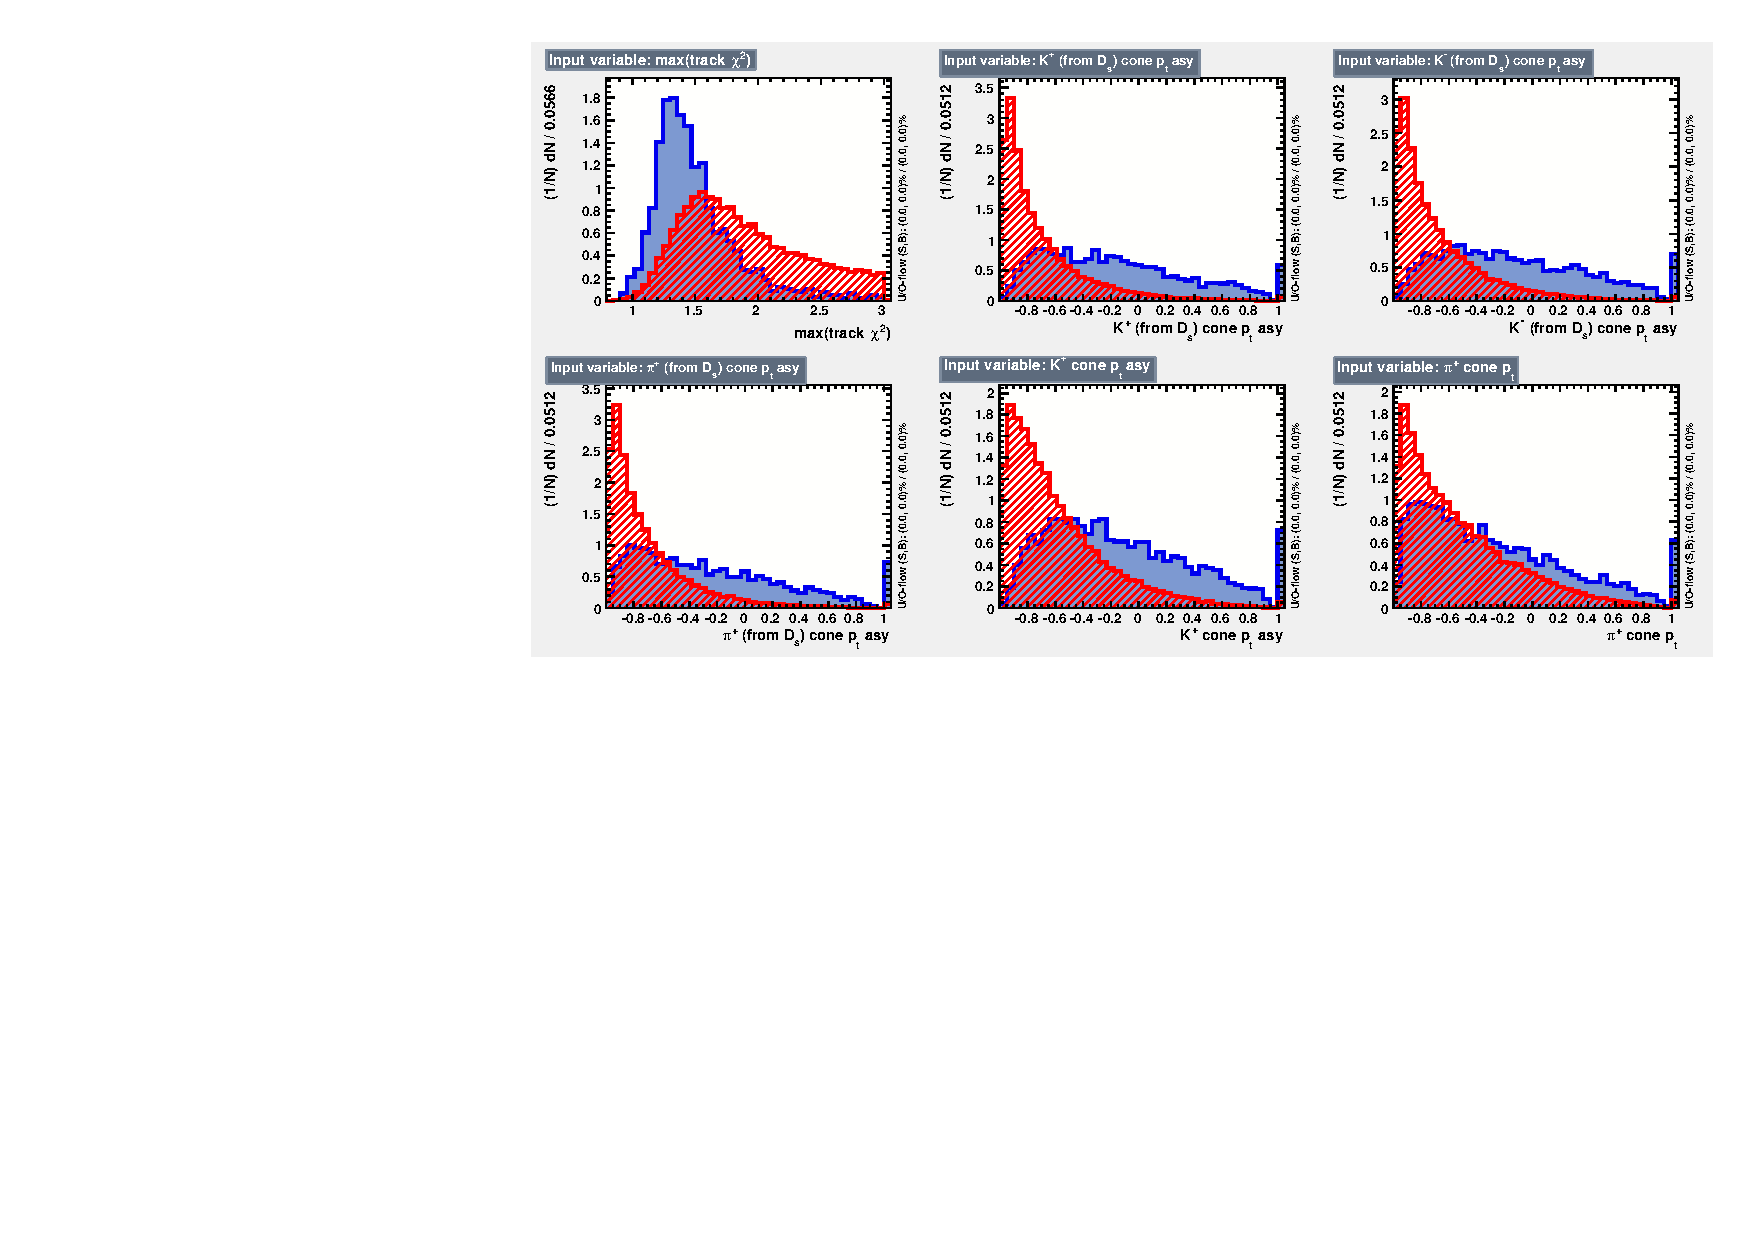
\includegraphics[width=10.0cm,height=5.5cm]{pics/BDT_Input_12_3}
\end{figure}

\end{frame}

\begin{frame}
\frametitle{BDT Input 4}

\begin{figure}
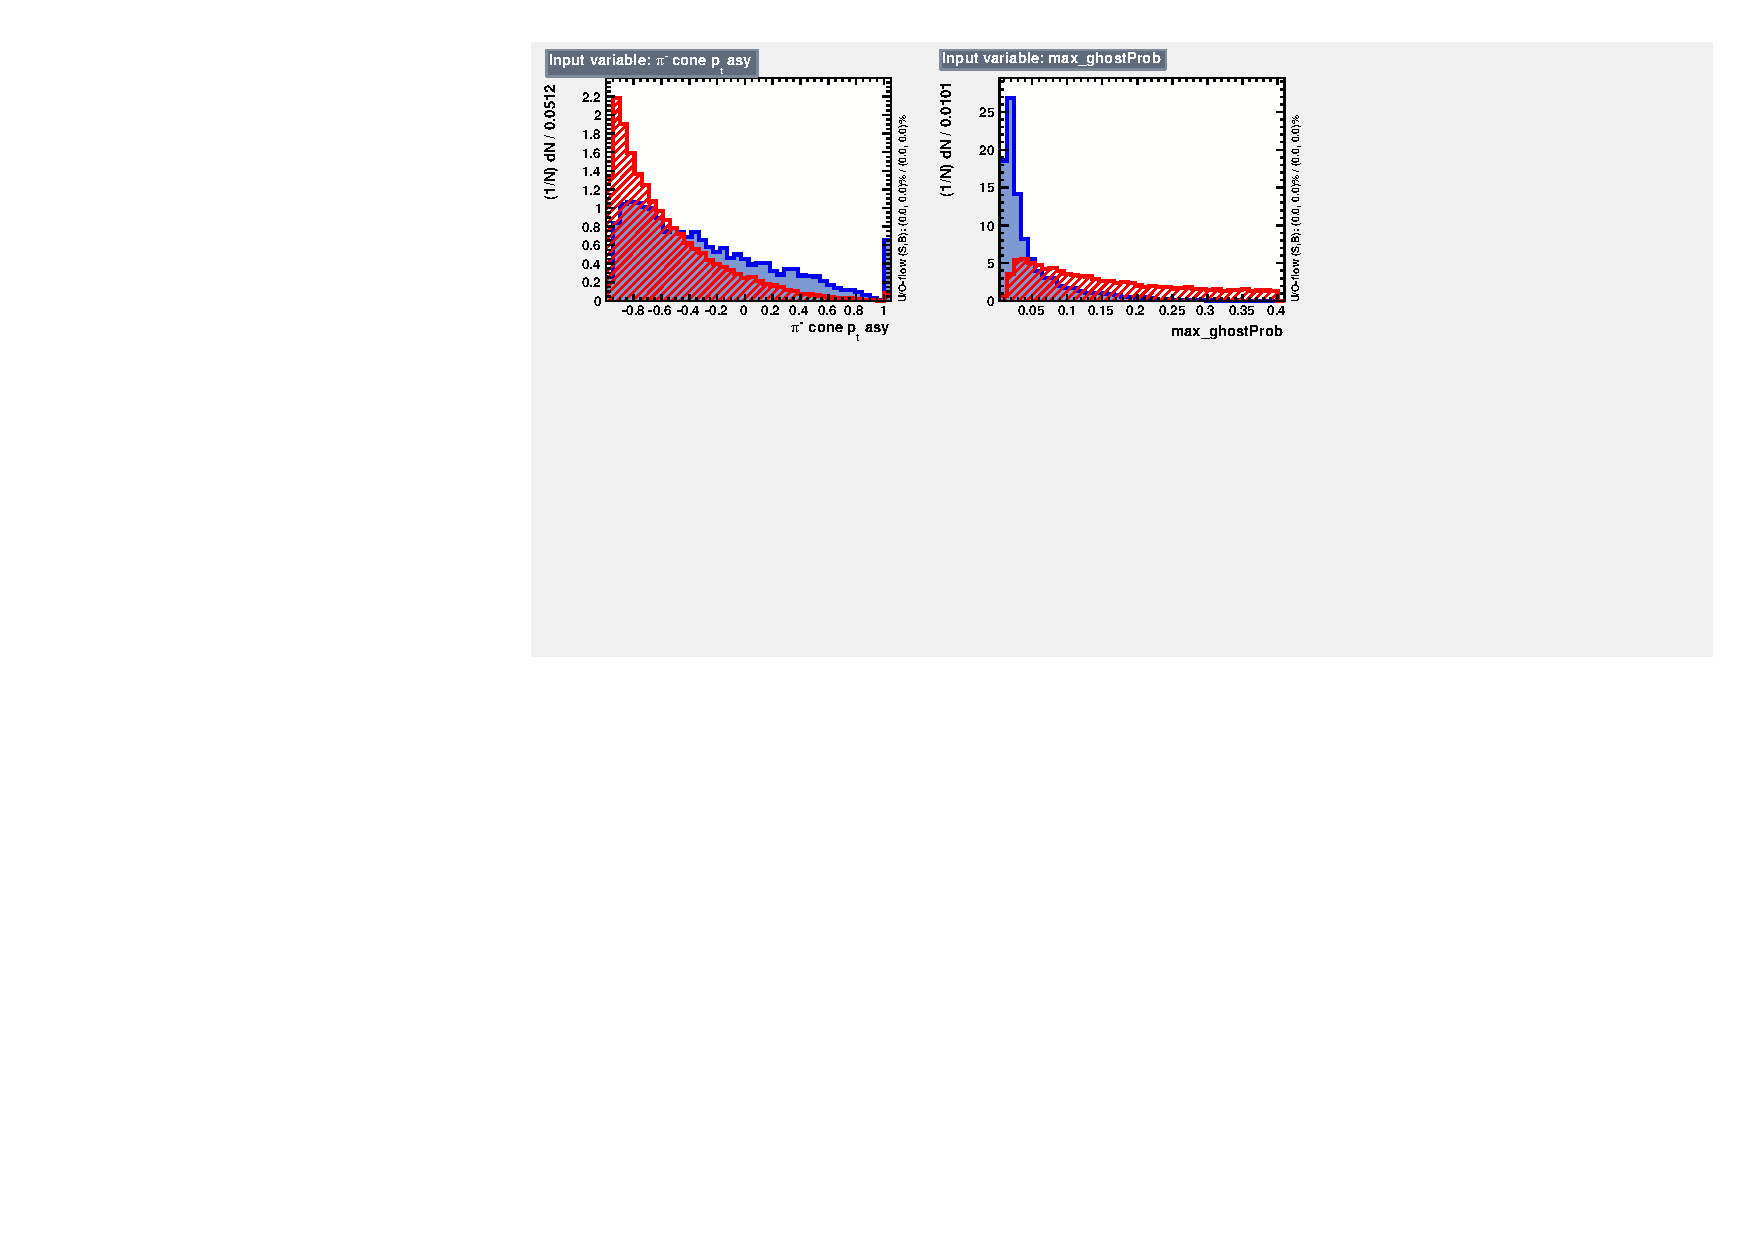
\includegraphics[width=10.0cm,height=5.5cm]{pics/BD_Input_12_4}
\end{figure}

\end{frame}

\begin{frame}
\frametitle{BDT Input correlation Signal}

\begin{figure}
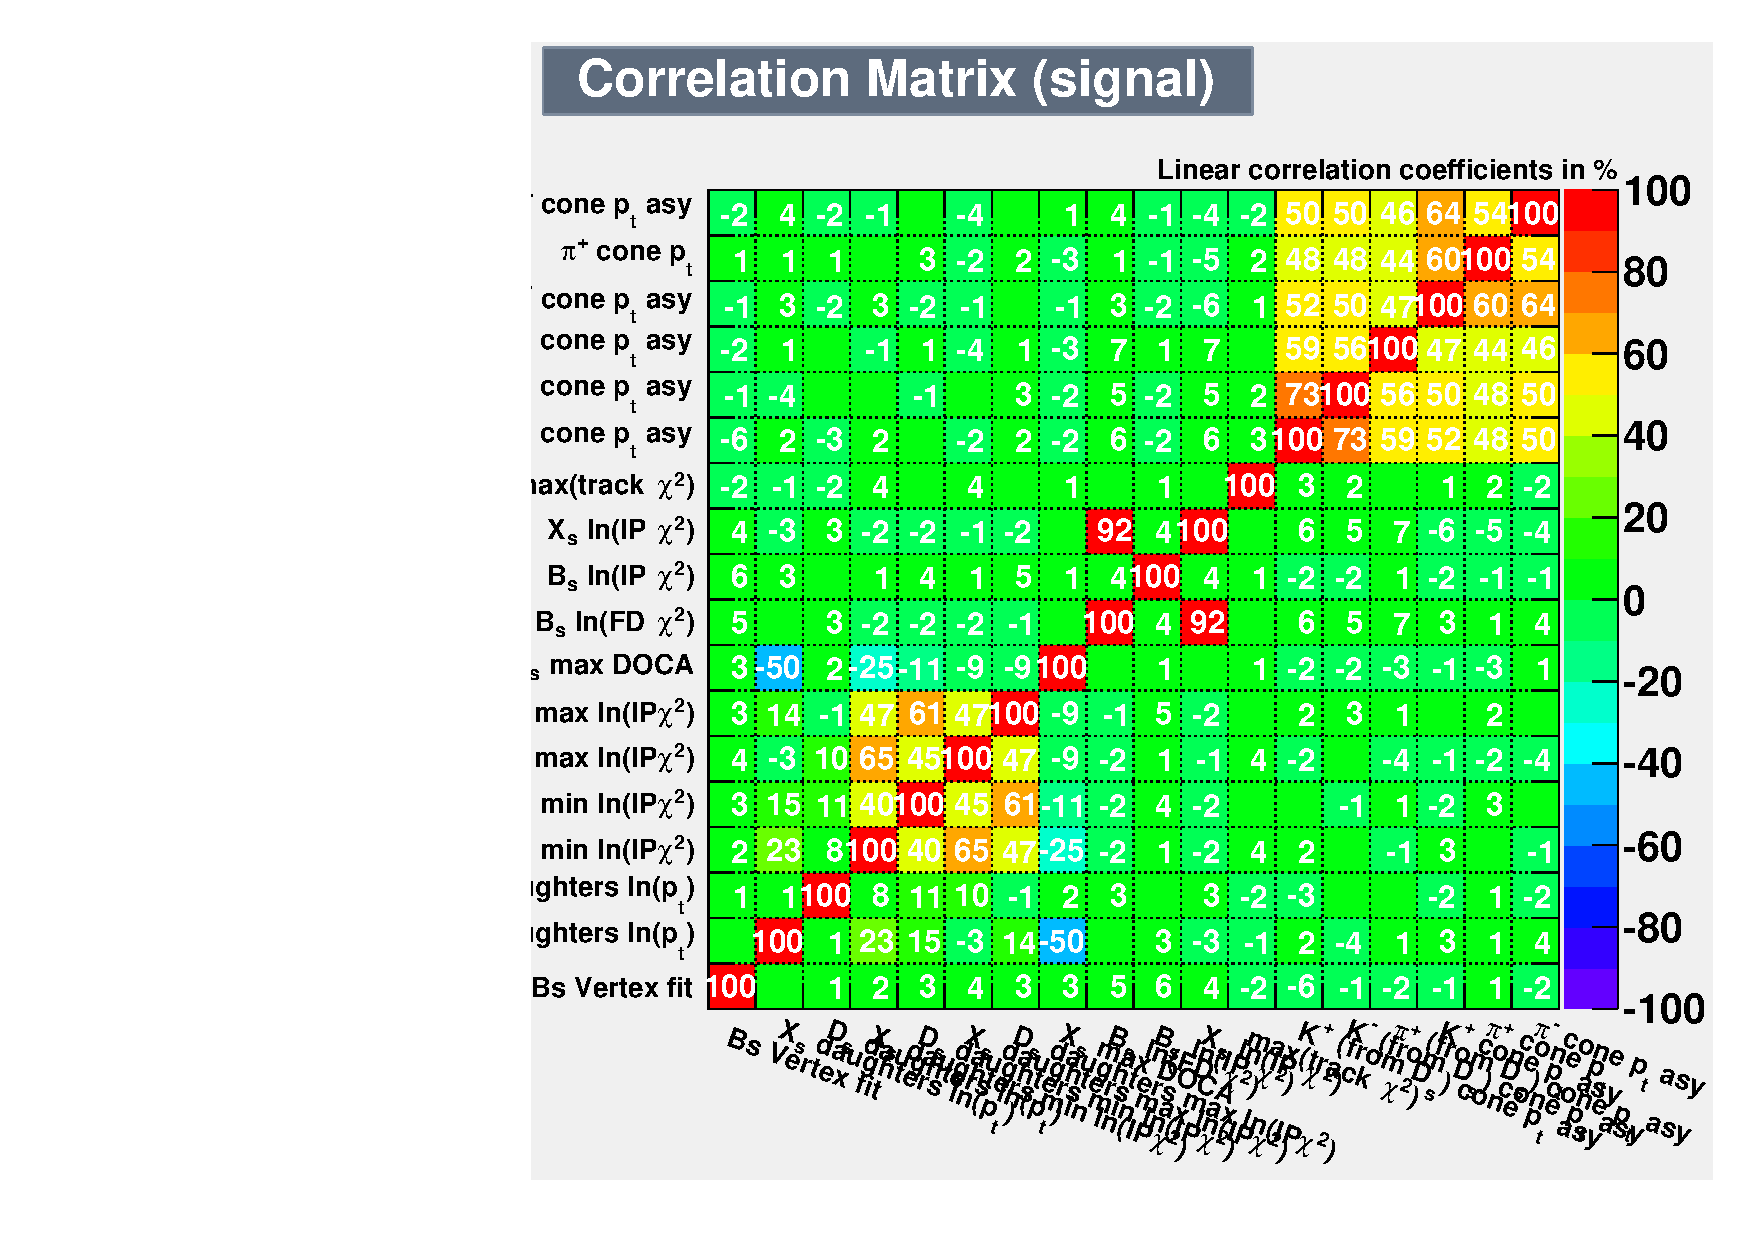
\includegraphics[width=10.0cm,height=7.5cm]{pics/BDT_correlation_signal}
\end{figure}

\end{frame}


\begin{frame}
\frametitle{BDT Input correlation Background}

\begin{figure}
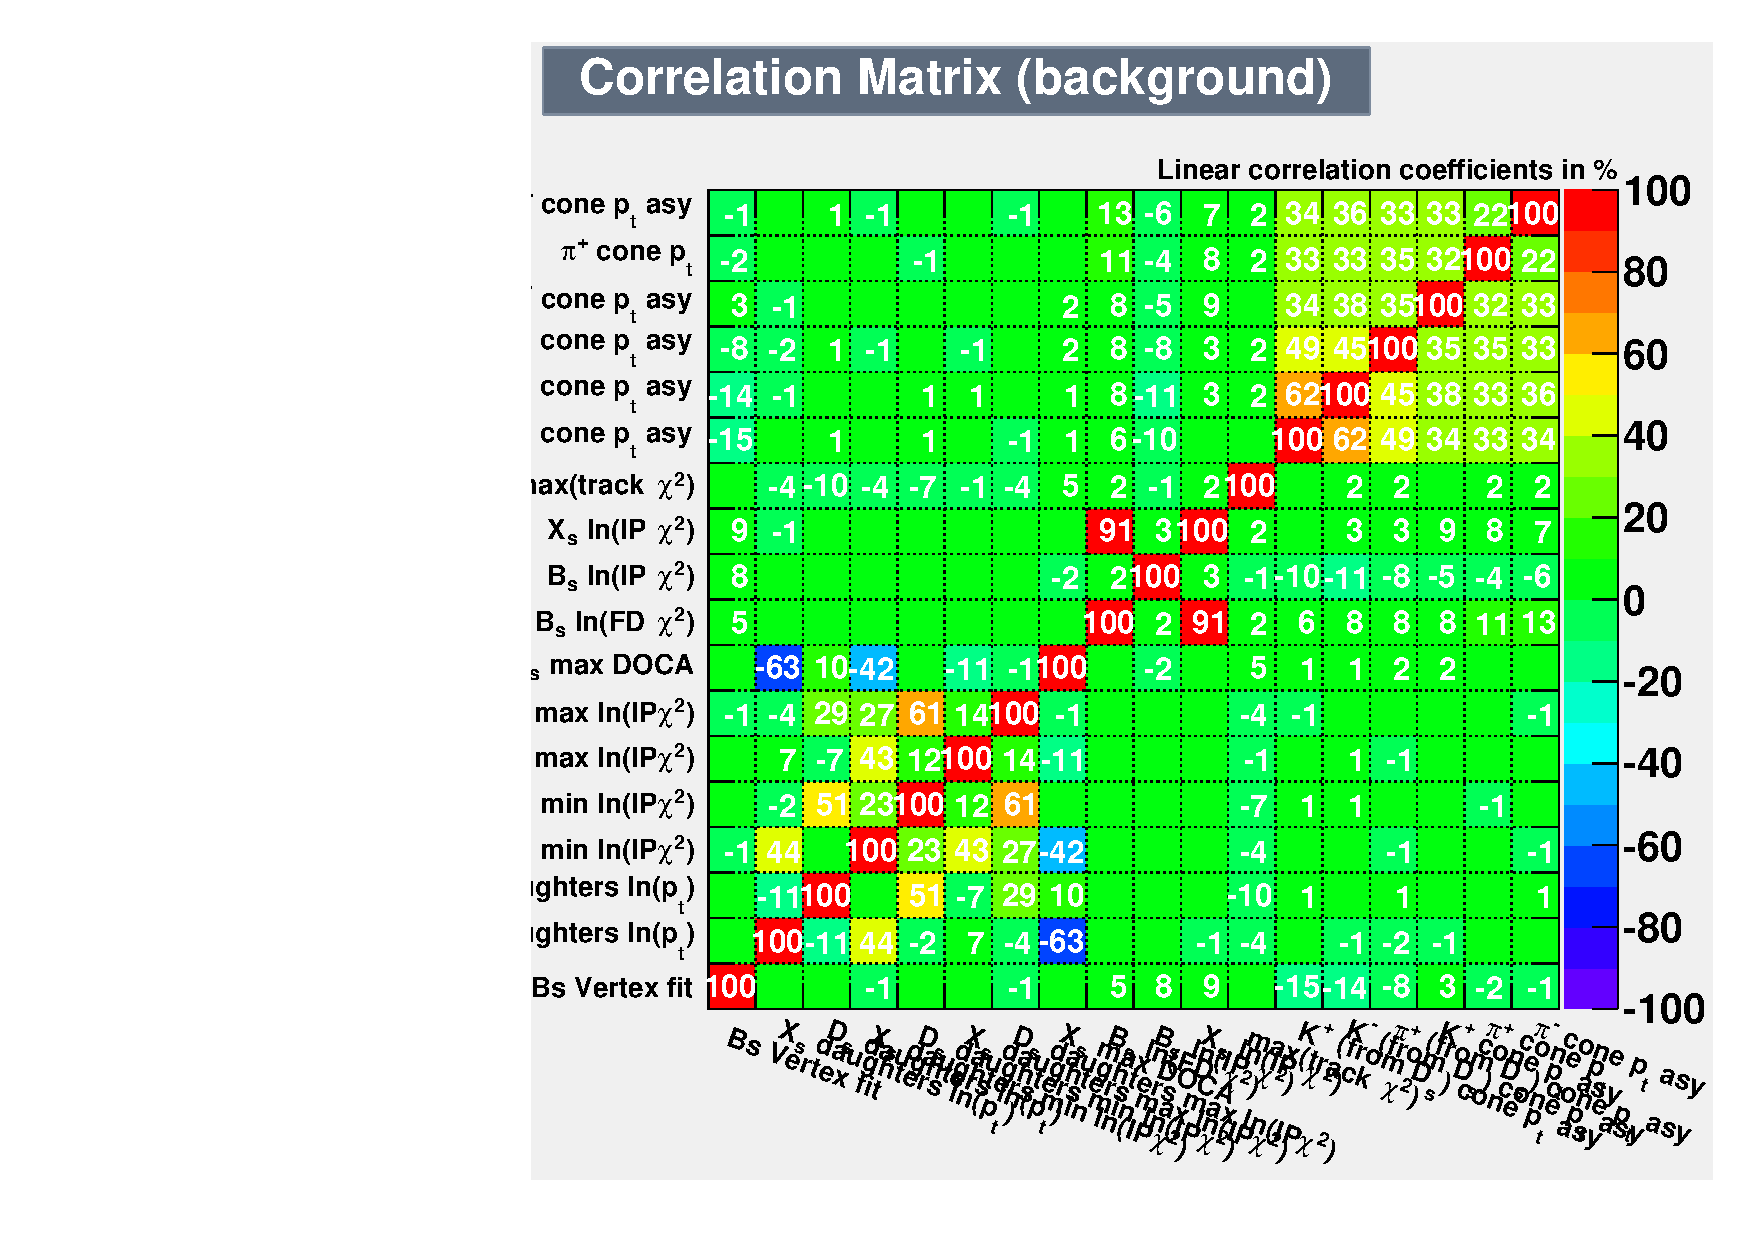
\includegraphics[width=10.0cm,height=7.5cm]{pics/BDT_correlation_background}
\end{figure}

\end{frame}

\begin{frame}
\frametitle{Time-dependent $\gamma$ determination}

%The decay rate for $B_{s}\to D_{s}^{-}K^{+}\pi^{+}\pi^{-} \equiv B_{s}\to f$ is:

\begin{equation*}
\begin{split}
\frac{d\Gamma_{B_{s}\to f}(t)}{dt} = \frac{1}{2}(1+|\lambda_{f}|^{2})e^{-\Gamma_{s}t} & [\cosh(\frac{\Delta\Gamma_{s}t}{2}) - \textcolor{green}{D_{f}}\sinh(\frac{\Delta\Gamma_{s}t}{2}) \\
& + \textcolor{red}{C_{f}}\cos(\Delta m_{s}t) - \textcolor{blue}{S_{f}}\sin(\Delta m_{s}t),]
\end{split}
\end{equation*}

with coefficients:

\begin{eqnarray*}
&\textcolor{green}{D_{f}} = \frac{2r_{D_{s}K\pi\pi}\cos(\Delta-(\gamma-2\beta_{s}))}{1 + r_{D_{s}K\pi\pi}^{2}}, 
\textcolor{red}{C_{f}} = \frac{1 - r_{D_{s}K\pi\pi}^{2}}{1 + r_{D_{s}K\pi\pi}^{2}}, \\
&\textcolor{blue}{S_{f}} = \frac{2r_{D_{s}K\pi\pi}\sin(\Delta-(\gamma-2\beta_{s}))}{1 + r_{D_{s}K\pi\pi}^{2}},
\end{eqnarray*}

with: \newline
$r_{D_{s}K\pi\pi} = \frac{A(\overline{B_{s}}\to D_{s}^{-}K^{+}\pi^{-}\pi^{+})}{A(B_{s}\to D_{s}^{-}K^{+}\pi^{-}\pi^{+})} = $ ratio of decay amplitudes and \\
$\Delta = $ strong phase difference \newline
\bfseries both vary over phase space \normalfont

\end{frame}


\end{document}